%% Based on a TeXnicCenter-Template by Tino Weinkauf.
%%%%%%%%%%%%%%%%%%%%%%%%%%%%%%%%%%%%%%%%%%%%%%%%%%%%%%%%%%%%%

%%%%%%%%%%%%%%%%%%%%%%%%%%%%%%%%%%%%%%%%%%%%%%%%%%%%%%%%%%%%%
%% HEADER
%%%%%%%%%%%%%%%%%%%%%%%%%%%%%%%%%%%%%%%%%%%%%%%%%%%%%%%%%%%%%
\documentclass[a4paper,twoside,11pt]{article}
% Alternative Options:
%	Paper Size: a4paper / a5paper / b5paper / letterpaper / legalpaper / executivepaper
% Duplex: oneside / twoside
% Base Font Size: 10pt / 11pt / 12pt


%% Language %%%%%%%%%%%%%%%%%%%%%%%%%%%%%%%%%%%%%%%%%%%%%%%%%
\usepackage[USenglish]{babel} %francais, polish, spanish, ...
\usepackage[T1]{fontenc}
%%\usepackage[ansinew]{inputenc}

\usepackage{lmodern} %Type1-font for non-english texts and characters

%% NG: Try the following for sans serif.
%% Well - take your pick. helvet leaves math in serif. But is otherwise rather nice?
\usepackage[scaled]{helvet}
%%\usepackage[math]{kurier}  %% Not nice.
%%\usepackage[math]{iwona}   %% Not nice.
%%\usepackage{cmbright}      %% Still will not work after installing hfbright.
\renewcommand*\familydefault{\sfdefault}

\usepackage{eulervm}
\usepackage{url}

%% NG: Try this for colour.
\usepackage{color}

\usepackage{float}

%% NG: Try this for HTML output
%% Also choose LaTeX => HTML of course ...
%%\usepackage[html]{tex4ht}

%% Packages for Graphics & Figures %%%%%%%%%%%%%%%%%%%%%%%%%%
\usepackage{graphicx} %%For loading graphic files
%\usepackage{subfig} %%Subfigures inside a figure
%\usepackage{tikz} %%Generate vector graphics from within LaTeX

%% Please note:
%% Images can be included using \includegraphics{filename}
%% resp. using the dialog in the Insert menu.
%% 
%% The mode "LaTeX => PDF" allows the following formats:
%%   .jpg  .png  .pdf  .mps
%% 
%% The modes "LaTeX => DVI", "LaTeX => PS" und "LaTeX => PS => PDF"
%% allow the following formats:
%%   .eps  .ps  .bmp  .pict  .pntg

%% NG: Try this to scale graphics to be at most the line length wide.
%% \includegraphics[width=\maxwidth]{figure}
\makeatletter
\def\maxwidth{%
  \ifdim\Gin@nat@width>\linewidth
    \linewidth
  \else
    \Gin@nat@width
  \fi
}
\makeatother

%% NG: Try fancy chapter headings.
%% This is Ulf Lindgren's FncyChap package. But set to Sans.
%\usepackage[Lenny]{fncychap}
%\ChTitleVar{\Huge\bfseries\sf}
%\usepackage[Glenn]{fncychap}
%\ChTitleVar{\Large\bfseries\sf}

%% NG: And we might want text in a box.
\usepackage{boxedminipage}

%% Math Packages %%%%%%%%%%%%%%%%%%%%%%%%%%%%%%%%%%%%%%%%%%%%
\usepackage{amsmath}
\usepackage{amsthm}
\usepackage{amsfonts}
\usepackage{mathrsfs}


%% Line Spacing %%%%%%%%%%%%%%%%%%%%%%%%%%%%%%%%%%%%%%%%%%%%%
%\usepackage{setspace}
%\singlespacing        %% 1-spacing (default)
%\onehalfspacing       %% 1,5-spacing
%\doublespacing        %% 2-spacing


%% Other Packages %%%%%%%%%%%%%%%%%%%%%%%%%%%%%%%%%%%%%%%%%%%
\usepackage{a4wide} %%Smaller margins = more text per page.
\usepackage{fancyhdr} %%Fancy headings
%\usepackage{longtable} %%For tables, that exceed one page

%% NG: Fancy verbatim text
\usepackage{relsize,fancyvrb}

%% NG: Font for Creative Commons license thing
\usepackage{cclicenses}

%% NG: Try barcodes (crumbs!)
%\usepackage{pst-barcode,pstricks-add}

%% NG: Node diagrams
\usepackage{pstricks,pst-node}

%% NG: Source code listings
\usepackage{listings,color}
\lstloadlanguages{Python,bash}
\lstdefinestyle{cp}{
  language=Python,
  frame=single,
  showstringspaces=false,
  basicstyle=\footnotesize\ttfamily
}
\lstdefinestyle{sh}{
  language=bash,
  frame=single,
  showstringspaces=false,
  basicstyle=\footnotesize\ttfamily
}
\lstdefinestyle{cpt}{
  language=Python,
  frame=single,
  showstringspaces=false,
  basicstyle=\tiny\ttfamily
}
\lstset{style=sh}

%% Index
%\usepackage{makeidx}
%\makeindex


%%%%%%%%%%%%%%%%%%%%%%%%%%%%%%%%%%%%%%%%%%%%%%%%%%%%%%%%%%%%%
%% Remarks
%%%%%%%%%%%%%%%%%%%%%%%%%%%%%%%%%%%%%%%%%%%%%%%%%%%%%%%%%%%%%
%
% TODO:
% 1. Edit the used packages and their options (see above).
% 2. If you want, add a BibTeX-File to the project
%    (e.g., 'literature.bib').
% 3. Happy TeXing!
%
%%%%%%%%%%%%%%%%%%%%%%%%%%%%%%%%%%%%%%%%%%%%%%%%%%%%%%%%%%%%%

%%%%%%%%%%%%%%%%%%%%%%%%%%%%%%%%%%%%%%%%%%%%%%%%%%%%%%%%%%%%%
%% Options / Modifications
%%%%%%%%%%%%%%%%%%%%%%%%%%%%%%%%%%%%%%%%%%%%%%%%%%%%%%%%%%%%%

%\input{options} %You need a file 'options.tex' for this
%% ==> TeXnicCenter supplies some possible option files
%% ==> with its templates (File | New from Template...).
\newcommand{\newpara}{\par\vspace{4mm}\noindent}
\newcommand{\myldots}{\ldots\ }

\addto\captionsUSenglish{\renewcommand*\abstractname{Summary}}

% Let us try bold text in red ...
\definecolor{OurRed}{rgb}{0.9,0.1,0.1}
\newcommand{\textbfc}[1]{\textbf{\textcolor{OurRed}{#1}}}
\newcommand{\textttc}[1]{\texttt{\textcolor{OurRed}{#1}}}
\newcommand{\textc}[1]{\textcolor{OurRed}{#1}}

% And in green ...
\definecolor{OurGreen}{rgb}{0.1,0.5,0.1}
\newcommand{\textbfg}[1]{\textbf{\textcolor{OurGreen}{#1}}}

% Alter some LaTeX defaults for better treatment of figures:
    % See p.105 of "TeX Unbound" for suggested values.
    % See pp. 199-200 of Lamport's "LaTeX" book for details.
    %   General parameters, for ALL pages:
    \renewcommand{\topfraction}{0.9}	% max fraction of floats at top
    \renewcommand{\bottomfraction}{0.8}	% max fraction of floats at bottom
    %   Parameters for TEXT pages (not float pages):
    \setcounter{topnumber}{2}
    \setcounter{bottomnumber}{2}
    \setcounter{totalnumber}{4}     % 2 may work better
    \setcounter{dbltopnumber}{2}    % for 2-column pages
    \renewcommand{\dbltopfraction}{0.9}	% fit big float above 2-col. text
    \renewcommand{\textfraction}{0.07}	% allow minimal text w. figs
    %   Parameters for FLOAT pages (not text pages):
    \renewcommand{\floatpagefraction}{0.7}	% require fuller float pages
	% N.B.: floatpagefraction MUST be less than topfraction !!
    \renewcommand{\dblfloatpagefraction}{0.7}	% require fuller float pages

%% argmin math operator    
\DeclareMathOperator*{\argmin}{\arg\!\min}

%% Choose to include the giant COMP figures or NOT.
\newif\ifinclcomp
\inclcompfalse
%%\inclcomptrue

    
\usepackage[xetex,unicode,
	pdftitle={GPLOT: A DIMFILM Based Graph Plotting Program for CDC NOS 2.8},
	pdfauthor={Nick Glazzard},
	colorlinks,linkcolor=blue,citecolor=blue,urlcolor=blue
	]{hyperref}

%%%%%%%%%%%%%%%%%%%%%%%%%%%%%%%%%%%%%%%%%%%%%%%%%%%%%%%%%%%%%
%% DOCUMENT
%%%%%%%%%%%%%%%%%%%%%%%%%%%%%%%%%%%%%%%%%%%%%%%%%%%%%%%%%%%%%
\begin{document}

\title{\textbf{GPLOT}: A \textbf{DIMFILM} Based Graph Plotting Program \\ for CDC NOS 2.8}
\author{Nick Glazzard}
%%\date{November 20, 2012}
\maketitle


%%\begin{abstract}
%%Stuff
%%\end{abstract}

%%\clearpage

%%\tableofcontents

%%\clearpage

\section{Introduction}
\textbf{GPLOT} is an interactive graphics program primarily focussed on graph plotting from data files.
It is based on U.L.C.C. \textbf{DIMFILM}, a substantial graphics library written and maintained
by Dr. John Gilbert between 1973 and approximately 1993. The version of \textbf{DIMFILM} used is
from somewhere around 1984 and is the second major version, which moved away from CDC Fortran
to portable, standard Fortran-77 (necessitated by U.L.C.C.'s move to Amdahl IBM compatible machines). 
\newpara
\textbf{GPLOT}, in contrast, is deliberately written for the CDC \texttt{FTN5} compiler under NOS 2.8 and
is not intended to be portable. It uses seven letter identifiers, dynamic memory allocation (via
the Common Memory Manager), and makes free use of NOS system calls.
\newpara
That said, it can be built and used on ``Unix-like'' systems (Debian Linux and macOS have been tested)
where it behaves almost identically to the NOS version.
\newpara
In overall intent, \textbf{GPLOT} is like a stripped down Gnuplot. 
\textbf{GPLOT} relies on character
string parsing subroutines written by Dr. Adrian Clark circa 1985. Dr. Clark also wrote a \textbf{DIMFILM} device
driver for Tektronix storage tube terminals on which the \textbf{GPLOT} Tektronix and, to some extent, \textbf{GTerm}, support
is based.
\newpara
The primary `interactive' output device for \textbf{GPLOT} is \textbf{GTerm} -- a simple terminal emulator with colour graphics
capabilities written in Python (see the \textbf{GTerm} project repository for more information). \textbf{GPLOT} also 
supports Tektronix 401x terminals (which \texttt{xterm} emulates, although Ren\'{e} Richarz's
excellent 4014 emulator is preferred).
\newpara
Output in the form of graphics files which  can be included in other documents is available in two formats:
Encapsulated PostScript files and SVG files. The latter is 
used by the \textbf{PMDHTML} Markdown to HTML program and the \textbf{PLNOTES} short document maintenance scheme for NOS
(which is not described further here) as well as for HTML documents in general. The former is useful for \LaTeX and other
`print' style document systems.
\newpara
\textbf{GPLOT} is currently at version 0.6. The first usable version (0.1, late 2013) 
could not output EPSF files as such, but used a
limited character set format that could be trivially translated to EPSF. V0.2 (2022) improved Tektronix 401x support. V0.58
(developed between late 2022 and early 2023) added significant -- if idiosyncratic -- facilities for function evaluation 
and other programmability features, as well as SVG output. It also exposed a lot more of DIMFILM's capabilities and directly
generated "true" EPS files. Most of what can be done with DIMFILM using a specially
written Fortran program can now be done from \textbf{GPLOT}. V0.59 fixed some bugs in parameter substitution. V0.6 (July 2025)
tidied up a few things and supported building on ``Unix-like'' systems as well as NOS. This version also uses the NOS MODIFY --
Git inter-operability tools so that the source can be managed equally well on NOS or with Git, with changes made on one system
being automatically reflected in the other. This version also automatically generates minor variations of the source code
needed for building on COS and Unix, using a single, NOS compatible, code base.
\newpara
A major goal for \textbf{GPLOT} is that it should be \textit{very easy to use} --- as easy as other graph plotting
programs on modern operating systems (such an Gnuplot, matplotlib, etc.) --- although \textbf{GPLOT} will never rival
the full capabilities of those systems.
\newpara
To build and install \textbf{GPLOT} on an emulated CYBER mainframe (with DtCyber), or on a ``Unix-like'' system,
please refer to the main \textbf{GPLOT} Github project \texttt{README.md}.

\section{Running \textbf{GPLOT}}
\textbf{GPLOT} needs two files: \texttt{GPLOT} (the pre-loaded binary executable) 
and \texttt{DADIMFO} (which contains
the font data for \textbf{DIMFILM}). To run \textbf{GPLOT} use:
\begin{verbatim}
/ATTACH,GPLOT.
/GPLOT.
\end{verbatim}
\texttt{GPLOT} will \texttt{ATTACH} the font file (\texttt{DADIMFO}) itself.
\newpara
The following control card options are recognized.
\begin{itemize}
\item \textttc{OBEY=FILE}\\
   \textbf{GPLOT} will start reading commands from the specified \texttt{LOCAL} file with name \texttt{FILE}. 
   The current version exits when the file
   has been read, but this might change in future versions.
\item \textttc{PARM=STRING}\\
   Used with \texttt{OBEY=FILE}. \texttt{STRING} is passed as one or more parameters to the \texttt{OBEY} file.
    See \ref{obfile} for more details.
   Under NOS, if \texttt{STRING} needs to contain spaces (i.e. there is more than one parameter), it should be enclosed in
   \$ signs. If any single parameter in \texttt{STRING} itself needs to contain spaces, that parameter should be enclosed in
   single quotes.
\item \textttc{GET=YN}\\
   Turn on automatic \texttt{GET}s of indirect \texttt{PERMANENT} files before \texttt{READ} and \texttt{OBEY} 
   try to access the files they need. \texttt{YN} is
   \texttt{YES} or \texttt{NO} (or an abbreviation down to \texttt{Y} or \texttt{N}). 
   This saves having to issue \texttt{GET} in \textbf{GPLOT} (or NOS before \textbf{GPLOT} is
   run) in order to make the files to be used \texttt{LOCAL}. On the other hand, if changes have been made to a \texttt{LOCAL} version
   of a \texttt{PERMANENT} file, these will be lost when \textbf{GPLOT} \texttt{READs} or \texttt{OBEYs} 
   that file with `auto \texttt{GET}' in effect. So be 
   careful!
\item \textttc{DEBUG=YN}\\
   Outputs debugging information (mostly to do with \texttt{OBEY} file arguments and parameter substitutions currently).
\item \textttc{QUIET=YN}\\
   Displays the unabbreviated command and \texttt{OBEY} nesting level for every command executed. Note that this may
   upset some output devices (it seems).
\item \textttc{SLIDE=YN}\\
	Tell DIMFILM to use a graph plotting layout suitable for slides. This is the default, as it seems better suited to most
	output devices. The alternative tends to have text and other features that look too small on the page or display. Some
	people might like that, though. 
\end{itemize}
An example of a \textbf{GPLOT} control statement is:
\begin{verbatim}
GPLOT,OBEY=DOPLOT,PARM=$X Y 'A TITLE'$.
\end{verbatim}

\begin{quote}
\begin{center}
\textbf{Note}\\
\end{center}
\textbf{GPLOT} can be run as any other command on ``Unix-like'' systems, but the current directory
must contain the fonts file \texttt{DADIMFO} when the command is issued otherwise \textbf{GPLOT} will
immediately exit with an error message. To avoid this problem, run \textbf{GPLOT} via the script \texttt{ugplot}
which arranges things so that this problem is avoided.
\end{quote}

\section{Commands}
All commands can be abbreviated so long as they uniquely identify a command.
(If the abbreviation is ambiguous, you will get a warning message and no command will
be executed). 
\newpara
All commands are shown in \texttt{UPPER CASE}, as that is the primary (\texttt{NORMAL}) character mode
for NOS. In \texttt{NORMAL} mode, lower case is equivalent to upper case, so lower case can be used
if desired. 

\begin{quote}
\begin{center}
\textbf{Warning}\\
\end{center}
\textbf{GPLOT} should
\textit{not} be used in \texttt{ASCII} mode on NOS (in which lower case characters are \textit{really} lower case),
otherwise command names will not be recognised, amongst other problems.
This does not mean that lower case text cannot be plotted, though -- it can.

\newpara
On ``Unix-like'' systems, lower case input can be used freely. Command names are converted to upper case internally.
Strings and file names preserve the case as entered. Also, EPS and SVG output files are given their usual extensions
(extensions are alien to NOS and COS). However, RPN evaluator operator names must still be given in
upper case.
\end{quote}

\newpara
Commands are divided in to related groups below, but that is only for 
convenience in describing them.

\subsection{Basic Graphics Commands}
These are the lowest level facilities on which graph plotting is built.
\begin{itemize}
\item \textttc{DEVICE NAME [OUTPUT-FILE]} --- Select the output device.\\
   The EPS and SVG devices need an output file name to write to. Note that this
   will be created as a \texttt{LOCAL} file and will need to be made permanent with
   \texttt{SAVE} or \texttt{REPLACE} on NOS. See Section \ref{devinfolabel} for the available devices and their
   characteristics.
\item \textttc{CLEAR} --- Clear the drawing area.\\
   The device display will be set to its default background colour.
   Any previously drawn material will be erased. This is also required to flush output to files
   for the \texttt{EPSCOL} and \texttt{EPSBIN} devices.
\item \textttc{BOUNDS XL XH YL YH} --- Set the plotting bounds.\\
   This establishes a user coordinate system with $x_l,y_l$ at the bottom left
   and $x_h,y_h$ at the top right. The \texttt{MOVE}, \texttt{DRAW}, 
   \texttt{PANE} and \texttt{BLANK} commands use this
   coordinate system.
\item \textttc{PANE XL XH YL YH} --- Set the \texttt{PANE} (clipping area).\\
   All drawing with \texttt{MOVE}, \texttt{DRAW} and \texttt{TEXT} will be clipped to the area specified
   here. In contrast, all graph plotting commands will apply inside this area,
   so that graphs will be scaled to fit this region. This is a way to plot
   multiple graphs side by side.
\item \textttc{UNPANE} --- Stop using any pane.\\ 
   The full drawing area will be used after this.
\item \textttc{PANEOUTLINE} --- Outline the pane area.\\
   A rectangle is drawn that matches the pane area.
\item \textttc{BLANK XL XH YL YH} --- Set the blank area.\\
   No drawing with either the basic graphics or graph plotting routines will
   make a mark inside the specified area. This can be useful for reserving a
   space for a graph key, for example.
\item \textttc{UNBLANK} --- Stop using any blank area.\\
   The previous blank area is no longer protected after this.
\item \textttc{BLANKOUTLINE} --- Outline the blank area.\\
   A rectangle is drawn that matches the blank area.
\item \textttc{COLOUR R G B} --- Set the RGB colour to use for drawing.\\
   \textbf{DIMFILM} maintains a separate drawing colour and line width for three
   different classes of graphical objects: lines, including those on graph plots;
   text (character strings); and graph plot annotations. This \texttt{COLOUR}
   command will be applied to the colour/style group last selected with
   a \texttt{CSGROUP} command (all 3 groups being the default if \texttt{CSGROUP} hasn't
   been used).
\item \textttc{WIDTH WIDTH} --- Set the line width.\\
   The width is a multiple of a device dependent "base width" and not all devices
   can draw wide lines (currently, only the Tektronix device cannot). This \texttt{WIDTH} will
   apply to the currently selected colour/style group as explained for \texttt{COLOUR}.
\item \textttc{CSGROUP GROUPNAME} --- Set the current colour/style group.\\
	This chooses which class of graphical objects any subsequent \texttt{COLOUR} and \texttt{WIDTH}
	commands apply to. The \texttt{GROUPNAME} values are: 
	\begin{itemize}
	\item \textttc{ALL} -- Apply COLOUR and WIDTH to all three colour/style groups.
	\item \textttc{GENERAL} -- Apply them to line drawing operations.
	\item \textttc{TEXT} -- Apply them to text drawing operations.
	\item \textttc{ANNOT} -- Apply them to graph plot annotation operations.
	\end{itemize}
	As usual, these group names can be abbreviated, providing the abbreviation
	remains unique.
\item \textttc{STYLE STYLENAME} --- Set the line style.\\
   The following styles are defined: \texttt{SOLID}, \texttt{DASH},
   \texttt{DOT}, \texttt{DASHDOT}. These are
   probably self explanatory!
\item \textttc{MOVE X Y} --- Move to position.
   The virtual pen is moved to $(x,y)$ in \texttt{BOUNDS} coordinates.
\item \textttc{DRAW X Y} --- Draw to position.\\
   The virtual pen is lowered and moved to $(x,y)$ in \texttt{BOUNDS} coordinates.
\item \textttc{TEXT "TEXT"} --- Draw text.\\
   The string \texttt{TEXT} is drawn at the current pen position. The string may be enclosed
   in double quotation marks to allow spaces in the string. The text will be drawn
   with the current font, which defaults to \texttt{SANS.SIMPLEX}. The string may contain many special
   formatting sequences. The most frequently useful are \texttt{*L} to switch to lower case
   and \texttt{*U} to switch back to upper. The full set of format controls are described in
   the \textbf{DIMFILM} manual, and a summary of most of them is given in Table~\ref{tab:textformats}.
   On systems other than NOS, lower case letters will be preserved.
\item \textttc{FILL} --- Fill the drawing area with the current colour.\\
   This clears the graphics area to the current colour, erasing it. It differs from
   \texttt{CLEAR} in that \texttt{CLEAR} always fills with white and empties any buffered graphics commands
   in the device (if relevant). \texttt{FILL} is only really useful after a \texttt{CLEAR} though, as it
   destroys anything already drawn. This command is device dependent and isn't useful for all devices.
   Only \textbf{GTerm} supports it currently.
\end{itemize}

\begin{table}
\begin{footnotesize}
\centering
\begin{tabular}{|| l | l ||}
\hline
Sequence & Purpose \\
\hline
\texttt{*U} & Start upper case. This is the default state and \texttt{\$U} is not useful.\\
\texttt{*L  \ldots \$L} & Start and end lower case.\\
\texttt{*B} & Backspace over last character.\\
\texttt{*1} or \texttt{*2} or \texttt{*3} & Select a font set.\\
\texttt{*+  \ldots \$+ } & Start and end super-script. Maximum of 2 levels.\\
\texttt{*\_ \ldots \$\_} & Start and end sub-script. Maximum of 2 levels.\\
\texttt{*N} & Reset sub- or super- script level to zero.\\
\texttt{*O }\ldots \$O & Make sub- or super- scripts fully below or above previous character (for summations).\\
\texttt{*,} numerator \texttt{\$,} denominator \texttt{\$.} & Construct a fraction.\\
\texttt{*:nn} & Output current symbol font character with code number \texttt{nn} (00 to 96).\\
\texttt{*::nn} & Output current marker font character with code number \texttt{nn} (00 to 96).\\
\texttt{*Vnn }& Output current font set alphabetic character with code number \texttt{nn} (00 to 96).\\
\hline
\end{tabular}
\caption{Special text formatting character sequences}
\label{tab:textformats}
\end{footnotesize}
\end{table}

\subsection{Further Plotting Commands}
These add a small number of primitive shapes as well as more control over how text is drawn.

\begin{itemize}
\item \textttc{CIRCLE X Y R} -- Draw a circle.\\
	Centre at $(x,y)$ with radius $r$.
\item \textttc{ARC X Y R A1 A2} -- Draw an arc of a circle.\\
	Centre at $(x,y)$ and with radius $r$, starting at angle
	$a_1$ and ending at angle $a_2$. The angles are measured in degrees counter-clockwise from the positive X axis.
\item \textttc{RECT X Y W H} -- Draw a rectangle.\\
	With bottom left at $(x,y)$, width $w$, height $h$.
\item \textttc{CRECT X Y W H} -- Draw a rectangle.\\
	Centred on  $(x,y)$, width $w$, height $h$.
\item \textttc{FONT FONTNAME} -- Set the current font.\\
	The \texttt{FONTNAME} must be one of the alphabetic fonts listed by \texttt{LISTFONT}.
\item \textttc{SYMHT H} -- Set the height characters, symbols and markers.\\
	The height is given in user bounds units.
\item \textttc{SYMANG A} -- Set the angle at which text is drawn.\\
	The angle is in degrees measured counter-clockwise from the positive X axis.
\item \textttc{CTEXT W "TEXT"} -- Draw text centred at the current position.\\
	The text is scaled so its width is $w$ in user bounds units.
\end{itemize}

\subsection{Graph Axis Commands}
Before plotting a graph, \textbf{GPLOT} needs to know the range and type of the axes on which
to plot the graph. The default settings of \texttt{XYAUTO}, \texttt{XLINEAR} 
and \texttt{YLINEAR} mean that \textit{none}
of the commands below \textit{need} to be used before plotting, but you may want to use them. 
\begin{itemize}
\item \textttc{XYAUTO} --- Find both axis ranges automatically.\\
   \textbf{DIMFILM} will examine the range of the data in use when an \texttt{XYPOINT}, 
   \texttt{XYLINE} or \texttt{XYHISTOGRAM}
   command occurs and will set the axis ranges to match. Linear axes will be used.
\item \textttc{XYSAME} --- Keep the previous axis ranges.\\
   If a graph was plotted with \texttt{XYAUTO} on, and other graphs need to be plotted on the same
   axes, use \texttt{XYSAME} after the first graph has been drawn. 
\item \textttc{XRANGE XLO YHI} --- Set the X axis range.\\
   The X axis will run from \texttt{XLO} to \texttt{XHI}.
\item \textttc{YRANGE YLO YHI} --- Set the Y axis range.\\
   The Y axis will run from \texttt{YLO} to \texttt{YHI}.
\item \textttc{XLINEAR} --- Use a linear X axis.\\
   This is the default.
\item \textttc{YLINEAR} --- Use a linear Y axis.\\
   This is the default.
\item \textttc{XLOG} --- Use a logarithmic X axis.
\item \textttc{YLOG} --- Use a logarithmic Y axis.
\end{itemize}

\subsection{Graph Plotting Commands}
These are the commands that get the data to be graphed and actually draw graphs. Before data
can be plotted, it must be \texttt{READ}, so the graph drawing commands 
(\texttt{XYPOINT}, \texttt{XYLINE} and \texttt{XYHISTOGRAM})
will not work until a \texttt{READ} has got some data. The graphs that can be drawn depend on what
data is \texttt{READ} --- this can be two real numbers per point (for $(x,y)$), three -- which adds 
information for a symmetric Y error bar, or four -- which adds data needed for asymmetric Y
error bars, or symmetric Y and X error bars. The graph drawing commands will always use all
the data available, so if \texttt{READ} has got data for $(x,y)$ and a symmetric Y error bar, for example,
that is what \texttt{XYPOINT} and \texttt{XYLINE} will draw. To stop drawing unwanted items, simply re-read the
data omitting the undesired items.
\begin{itemize}
\item \textttc{MAXPOINTS NUMBER} -- Set maximum number of data points.\\ 
   Memory for data to be plotted is allocated dynamically (this could be
   done in most major Fortran implementations, even though it is completely non-standard
   in Fortran-77 and earlier --- there is much, possibly deliberate, ignorance on the part
   of academics of what could actually be done in this language). Four real numbers are allocated
   for each point --- two for an $(x,y)$ coordinate and two for error bar data. On starting,
   \textbf{GPLOT} allocates space for 1000 points. This can be changed at any time (although any data
   \texttt{READ} will be thrown away if it is changed, of course). The number of data points is limited
   by the amount of central memory on the machine, and how much of that you are allowed to use by
   your account settings. Under emulation, there is no reason not to use the maximum
   available --- 262,144 words of which 131,072 can be used by any one job (minus a bit, of
   course!). \textbf{GPLOT} is, unfortunately, not small ... and will grow as more facilities are
   added. At present, the maximum number of points allowed is set to 10000 and this is close to the
   maximum possible. The limit of addressable central memory is the main limitation on what
   can actually be done under NOS. Although extended memory and `out-of-core' solutions (where
   most of the data resides on disk) may be possible in some cases, that isn't always so (e.g.
   \textbf{DIMFILM} needs the data it plots to be in central memory), and these methods always come
   with a significant performance and complexity cost.
   \begin{quote}
     \begin{center}
       \textbf{Note}\\
       On ``Unix-like'' systems, this command has no effect. The default value is always used
       regardless of what may be specified here.
     \end{center}
   \end{quote}
\item \textttc{READ NAME XCOL YCOL [YECOL [XECOL]]} --- Read a data file using the specified `columns'.\\
   The file \texttt{NAME} (which must be a \texttt{LOCAL} file -- possibly obtained inside \textbf{GPLOT} using
   the \texttt{GET} command) should contain numbers (in the standard character code), with at least one per line,
   separated by spaces or commas. There may be any number of spaces preceding or separating each number
   (subject to line length limitations -- the limit may be 80). Blank lines are skipped and ignored.
   Lines with the character \texttt{`C'} in column 1 are ignored (allowing comments). 
   The \texttt{numbers} may be integers
   or any real number format (exponential or not), optionally preceded by a \texttt{+} or \texttt{-} sign. 
   \texttt{READ} will
   try to interpret anything that \textit{could} be a number \textit{as} a number. It will stop reading a data item
   when a non-numeric character is found --- but this is not treated as an error.\\
   Each space (or single
   comma) separated number on a line is termed a `column', and these are numbered starting at 1. So column
   2 is the second number on each line. Column numbers must be specified for \texttt{XCOL} and \texttt{YCOL} data to
   obtain at least an $(x,y)$ coordinate for each point. As a special case, \texttt{XCOL} may be 0, in which case,
   the X coordinate is set to the point number (starting at 1). This allows a data file with a single
   data item per line to be processed.\\
   If a column number is supplied for \texttt{YECOL},
   then that column's values will be used for symmetric Y error bars. If a column number is also specified
   for \texttt{XECOL}, then that data will be used as either a symmetric X error bar or as the upper part of an asymmetric
   Y error bar, depending on the setting made with the \texttt{ASYMYERRORBARS} command. The default is to interpret 
   \texttt{YECOL} and \texttt{XECOL} as the lower and upper extents of asymmetric Y error bars, as this may be more frequently
   useful, There is currently no way to draw asymmetric X error bars --- although this could be added if the
   storage of 6 numbers per point was acceptable (I'm not sure it is).\\
   If \texttt{NAME} is \texttt{HERE} (i.e. the string \texttt{HERE}), 
   then no data file is opened. Instead, \texttt{READ} tries to read data from
   the command input stream itself (\texttt{INPUT} or an \texttt{OBEY} file -- see below). 
   \texttt{READ} will stop reading data items
   when it finds a line that contains the string \texttt{EOF} as its only item. This facility is mostly to allow
   other programs to write a self contained \texttt{OBEY} file that executes a complete plotting task then exits \textbf{GPLOT}.
   A major anticipated application of this is plotting data from APL.
\item \textttc{MARKER NUMBER} --- Set the marker number to be used for points.\\
   This is a character number in \texttt{Font 9001}. Characters are associated
   with numbers 2 to 25, but with 5 and 11 omitted. Numbers 2, 3, 4, 8, 9, 19 and 20 are perhaps the most useful.
   Something may need to be done to improve this font or at least supply descriptive names for the markers!
\item \textttc{XYPOINT} --- Draw an XY graph with points.\\
   The points will be drawn with the last marker set with a \texttt{MARKER}
   command, or 3 (the default) if no \texttt{MARKER} command is used. 
   Depending on the data items \texttt{READ} and the \texttt{ASYMYERRORBARS}
   setting, symmetric Y, asymmetric Y or symmetric Y and X error bars will also be drawn.
\item \textttc{XYLINE} --- Draw an XY graph with lines.\\
   By default, data points will be joined with straight lines (linear
   interpolation -- of a kind) and in \texttt{SOLID} line style. The line style can be changed with the \texttt{STYLE} command.
   Cubic or quintic interpolation can be used between the data points to get smooth curves instead of straight lines.
   At least 3 points are required for cubic and 5 for quintic interpolation. If there are insufficient points, linear
   interpolation is used as a fall-back. The interpolation is as supplied by \textbf{DIMFILM} --- as always, whether it is appropriate
   depends on the data and its desired interpretation. I'm not certain exactly how \textbf{DIMFILM} comes up with the interpolation,
   although it is visually fine.
\item \textttc{XYHISTOGRAM} --- Draw an XY histogram.\\
   Bars (of a type determined by \texttt{HISTSTYLE} --- default: \texttt{ABUT}) 
   are drawn centered on the X coordinate and extending vertically
   from the $X=0$ axis to the Y coordinate. Error bar data (if any) is ignored.
\item \textttc{HISTSTYLE STYLENAME [WIDTH]} --- Sets the histogram bar style.\\
   \texttt{STYLENAME} is one of the following:
   \begin{itemize}
   \item \textttc{ABUT} --- Open rectangular bars are drawn, centred on an X coordinate, and with a width determined by the X location
   of the preceding point (apart from the first point, which uses the location of the second point), so that the bars touch one
   another along the X direction.
   \item \textttc{ABUT+SHADE} --- as \texttt{ABUT}, but the bars are filled with `shading' ---
   lines at 45 degrees spaced 0.02 of the X \texttt{BOUNDS} range
   apart.
   \item \textttc{LINES} --- Zero width lines are used for the bars.
   \item \textttc{WIDE} --- Bars of the specified \texttt{WIDTH} (in X axis units) are drawn without shading.
   \item \textttc{WIDE+SHADE} --- As \texttt{WIDE}, but with shading.
   \end{itemize}
\item \textttc{INTERPOLATE STYLE [N]} --- Set the interpolation mode for \texttt{XYLINE}.\\
   \texttt{STYLE} may be: \texttt{LINEAR}, \texttt{CUBIC} or \texttt{QUINTIC} --- which are hopefully self explanatory!
   As explained in \texttt{XYLINE}, either straight lines or smooth curves can join the points. 
   If \texttt{CUBIC} or \texttt{QUINTIC} is used, the
   number of intermediate (linear) segments drawn for the curve between each point is controlled by \texttt{N} (default: 10).
\item \textttc{ASYMYERRORBARS MODE} --- Use asymmetric Y error bars if \texttt{MODE} is \texttt{ON}.\\
   If \texttt{OFF}, symmetric Y and X error bars are drawn. Error bars will only be drawn if error bar
   data has been \texttt{READ}, and both \texttt{YECOL} and \texttt{XECOL} must have been 
   specified to get asymmetric Y error bars or
   symmetric Y and X error bars.
\end{itemize}


\subsection{Graph Annotation Commands}
Graphs almost always need some annotation. Minimal annotation is: ticks on the axes, numeric values
against those ticks, and a framing rectangle drawn around the graph plotting area. These are always
drawn after each graph drawing command (\texttt{XYPOINT}, \texttt{XYLINE}, \texttt{XYHISTOGRAM}) 
unless \texttt{ANNOTATE OFF} is used.
\texttt{TITLE}, \texttt{XLABEL}, \texttt{YLABEL} and \texttt{GRID} annotation elements are only 
drawn if these are explicitly specified.
\begin{itemize}
\item \textttc{ANNOTATE ON} or \texttt{OFF} --- Turn annotation on or off.\\
   Typically, annotation is wanted whenever a single graph is drawn. However, after drawing one curve
   (etc.) with annotation, it might be desirable to turn off annotation when drawing the other curves
   on the same axes. It is certainly more efficient to do so, and some devices with some line width settings
   may show visible changes when items are drawn over existing identical elements (for whatever reason).
\item \textttc{TITLE "TEXT"} --- Set the title.\\
   This is drawn at the top of the graph, centred on the width of the graph drawing area.
   \texttt{TEXT} may be enclosed in double quotes to allow spaces and format commands 
   (such as \texttt{*L} and \texttt{*U}) are
   understood.
\item \textttc{XLABEL "TEXT"} --- Set the X axis label.\\
   This is plotted below the X axis (at the bottom of the graph drawing area.
\item \textttc{YLABEL "TEXT"} --- Set the Y axis label.\\
   This is plotted (vertically) to the left of the Y axis.
\item \textttc{GRID Style} --- Draw a grid with lines at the major axis ticks for one or both axes.\\
   Style may be: \texttt{NONE}, \texttt{X}, \texttt{Y}, or \texttt{BOTH}, which are hopefully self explanatory.
   Note that the grid will only be drawn if \textttc{ANNOTATE ON} is in effect (it will not be  drawn if
   \textttc{RIGHTANNOT ON} is in effect).
\item \textttc{GSTYLE Mode} --- Choose the overall graph drawing style.  \\
	Mode may be:
	\texttt{BOXED}, \texttt{AXES} or \texttt{OPEN}. The default is \texttt{BOXED}, with axis annotations along the
	edges of a boxed region. The \texttt{OPEN} option disposes of the right and top edges.
	\texttt{AXES} draws only axis lines that pass through a point which can be specified but defaults to $(0,0)$. This
	gives a dramatically different appearance. Note that the point the axes pass through must be in the range of
	graph values to be drawn, otherwise one or both of the axes will be omitted..
\item \textttc{AXCUT X Y} --- Set the coordinates through which axis lines will pass. \\
	If using \texttt{GSTYLE AXES} this must
	be used to position the axes in the coordinate ranges being used, otherwise no annotation will appear.
\item \textttc{RIGHTANNOT ON} or \texttt{OFF} --- Selects annotation of the right hand edge for \texttt{GSTYLE BOXED}. \\
	This will
	only be drawn if \texttt{ANNOTATE OFF} has been previously used to stop left edge annotation. Using this with changes to 
	\texttt{YRANGE} allows data with different Y value ranges to be drawn on the same plot.
\item \textttc{ RYLABEL "TEXT"} --- Sets the right hand edge label.\\
	This is useful if \texttt{RIGHTANNOT ON} is used.
\end{itemize}

\subsection{\textbf{GPLOT} System Commands}
These commands don't draw anything, but they show the state of \textbf{GPLOT}, interact usefully with NOS, and allow
something like plotting macros (with parameters) to be used.
\begin{itemize}
\item \textttc{OBEY NAME [PARAMETERS]} --- Start reading commands from file \texttt{NAME}.\label{obfile}\\
   The file may contain any \textbf{GPLOT} command (one per line), including \texttt{OBEY}. \texttt{OBEY} files may be
   nested up to 5 deep (this could be increased, but 5 seems likely to be enough). If \texttt{PARAMETERS}
   is specified, it should be a single string without spaces or a string enclosed in double quotation
   marks. Each space separated word in the \texttt{PARAMETERS} string defines a single parameter, which are
   given numbers based on position starting at 1 on the left. Up to 9 parameters can usefully be set up
   in the \texttt{PARAMETERS} string. When reading commands from an \texttt{OBEY} file, \textbf{GPLOT} will apply a simple
   parameter substitution process: each space separated word of the form: \texttt{\$N}, where \texttt{N} 
   is \texttt{1} to \texttt{9}, will
   be replaced by the \texttt{N}th word of the \texttt{PARAMETER} string. It is possible to pass parameters containing spaces
   by enclosing them in single quotes in the \texttt{PARAMETER} string. For example:
   \begin{verbatim}
   OBEY FRED "FIRST 'SECONDA SECONDB'"
   \end{verbatim}
   defines two actual parameters that will be substituted for the formal parameters \texttt{\$1} and \texttt{\$2} wherever
   these occur as space separated words in the file FRED. \texttt{\$2} will, in fact, be substituted as:
   \begin{verbatim}
   "SECONDA SECONDB"
   \end{verbatim}
   in order to preserve the embedded space(s). This is useful for passing \texttt{TITLE} strings to \texttt{OBEY} files,
   for example.
\item \textttc{HELP} --- Outputs summary help information, including the supported output devices.
\item \textttc{STATUS} --- Displays various \textbf{GPLOT} state information.\\
   This includes the number of points available, whether anything has been read, the \texttt{BOUNDS}, whether
   any \texttt{PANE} or \texttt{BLANK} is in effect, etc.
\item \textttc{LOGFILE NAME} --- Opens a command log file called \texttt{NAME}.\\
   This is a \texttt{LOCAL} file to which any interactive input from you, the user, is written. Commands executed
   from any \texttt{OBEY} files are not logged. This lets you log a session and repeat it (perhaps after editing)
   by executing the log file as an \texttt{OBEY} file. You will need to \texttt{SAVE} or \texttt{REPLACE} the file to make it
   \texttt{PERMANENT} if you want to keep it between jobs. When \texttt{LOGFILE} is executed, any previously open log file
   is closed and a new one is opened. If the new one has a different name from the old, the old one will
   not be destroyed.
\item \textttc{MEMTEST} --- Test dynamic memory is working.\\
   Which it will be! More usefully, it also generates test data in the form of a sine wave, which can then
   be plotted to evaluate how well an output device is working, or to get familiar with \textbf{GPLOT}.
\item \textttc{GET NAME} --- Get an indirect access \texttt{PERMANENT} file.\\
   This is useful to avoid having to exit \textbf{GPLOT} to make some data file \texttt{LOCAL} so it can be \texttt{READ}.
   There is no command as yet to \texttt{ATTACH} a direct access \texttt{PERMANENT} file, although it would be easy
   to add one.
\item \textttc{LISTFONT} --- Lists the available fonts.\\
	The names of all available fonts are shown, along with the type of font: \texttt{ALPHABETIC}, \texttt{SYMBOL} or 
	\texttt{MARKER}. 
\item \textttc{EXIT} --- Exit \textbf{GPLOT}.\\
   This closes any log file, flushes graphics commands to the output device, and shuts down \textbf{DIMFILM}. 
   Then it exits \textbf{GPLOT} --- surprise!
\end{itemize}

\section{Defining and Using Functions}
The ability to define and use functions is based on an \textbf{RPN evaluator} for simplicity, where operands are held on a \textbf{stack}.
However, in this case, the values on the
stack are arrays, each containing up to \texttt{MAXPOINTS} elements. These stack entries may also be used to hold scalar values
as needed by the RPN operators. The scalar values are held in the first element of the arrays. 

\subsection{Overview, storage and RPN evaluator commands}
There are a number of \textbf{commands} associated with the RPN evaluator and these are like other \textbf{GPLOT} commands.
The RPN evaluator itself deals with \textbf{operators} which act on \textbf{operands} with an entire thing to be evaluated defined
as an \textbf{RPN-string} consisting of comma separated operands and operator names. The operand and operator name strings are
the two types of \textbf{tokens} understood by the RPN evaluator. 
\newpara
The size of the stack can be set with the command:
\begin{itemize}
\item \textttc{NSTACK n}
\end{itemize}
where \texttt{n} is an integer greater than or equal to 4. The default is 8. The number of words used by the stack is 
\texttt{NSTACK * MAXPOINTS}
and this must be compatible with the maximum field length. The first four stack entries are also used to store X and Y points 
and X and Y error bars for graph plotting, so \texttt{NSTACK} must be at least 4.
\newpara
The stack entries are numbered 0, 1 \ldots \texttt{NSTACK-1}. Stack entry 0 is special:
\begin{itemize}
\item It can only be written to by the \textttc{ERANGE} command or the \textttc{XLIN}, \textttc{XLOG} and \textttc{SETX} 
RPN operators.
\item Writing to it with \textttc{ERANGE}, \textttc{XLIN} or \textttc{XLOG} sets the evaluation range and the number of active elements in
the stack arrays -- i.e. the array length, \texttt{NELEM} for evaluation purposes\footnote{Also referred to as
\texttt{NEVAL} internal to \texttt{GPLOT}.}.
\item Its contents can be accessed by the \textttc{X} RPN operator.
\end{itemize}
It is usual for the contents of stack level 0 to define the values for which the function will be evaluated, which is why its contents
are accessed with the operator named \textttc{X}. Since the effective array length must be known for the vast majority of operators to
work, either the \textttc{ERANGE} command \emph{must be used before} any RPN is evaluated or the \textttc{XLIN} or \textttc{XLOG} 
operators must be used before any other RPN operators. The contents of stack level 0 will be called the \textbf{X range array.}
\newpara
Stack level 1 is also special in that it contains the Y values corresponding to the X values in the X range array when plotting graphs.
This may be referred to as the \textbf{Y value array}. There is an RPN operator which explicitly sets this by copying the contents of
the top-of-stack (TOS) array into it.
\newpara
There are RPN operators which directly produce graphical output. It is sometimes useful to know the bounds of that output before
actually drawing anything, and three commands are provided to do that.
\begin{itemize}
\item \textttc{BBSTART} prevents RPN operators that would normally draw things from doing so, but instead has them accumulate bounding
	box information.
\item \textttc{BBEND} restores normal operation of the graphics drawing RPN operators.
\item \textttc{BBSET} sets the bounds to the accumulated bounding box and is equivalent to issuing a BOUNDS command with the
	appropriate arguments.
\end{itemize}
\newpara
Three other groups of storage are also defined for use with function definition and evaluation:
\begin{itemize}
\item \textbf{Scalar Registers}: There are 9 registers (named 1 to 9) that can be used with \texttt{STO} and \texttt{RCL} commands and RPN
	operators to save scalar variables.
\item \textbf{String Registers}: There are 9 registers (named 1 to 9) to hold strings of up to 80 characters. These can be set with the
	\texttt{STRING} command and accessed by RPN operators.
\item \textbf{Procedure Registers}: These 9 registers (named 1 to 9) are used to hold RPN procedures as strings that can be `called`. The
	contents can be set with the command \texttt{PROC} to a literal string, or loaded from a procedure library file using the
	\texttt{LOADPROC} command (see below).
\end{itemize}
\newpara
A procedure is defined in the form of an \textbf{RPN-string} as a series of comma separated tokens:
\begin{verbatim}
TOKEN,TOKEN,...,TOKEN
\end{verbatim}
A \texttt{TOKEN} is a numeric constant operand or an RPN operator. Unlike commands, RPN operator names cannot be abbreviated. 
\newpara
There are two commands which can cause an \texttt{RPN-string} to be evaluated. The main one is:
\begin{itemize}
\item \textttc{EVAL RPN-string}
\end{itemize}
The \texttt{RPN-string} for EVAL can `call` procedures stored in Procedure Registers (as \texttt{RPN-string}s) using the token
\texttt{@n} where \texttt{n} is the Procedure Register number (1 to 9). This \texttt{@n}  token cannot be used in the \texttt{RPN-string}s)
stored in Procedure Registers, as a proper call stack is not maintained.
\newpara
A very useful variant on EVAL is:
\begin{itemize}
\item \textttc{ITEVAL start end step RPN-string}
\end{itemize}
which will evaluate the RPN-string \texttt{max( int( (end - start + step) / step ), 0 ) } times, as per a FORTRAN DO-loop. The value of
the loop counter can be accessed using the token \texttt{I} in the \texttt{RPN-string}. The \texttt{I} token has the value 1 if used in an
\texttt{RPN-string} evaluated via \texttt{EVAL}.

\subsection{How the RPN evaluator works}
The RPN evaluator's basic operation given an \texttt{RPN-string} is as follows:
\begin{enumerate}
\item Split \texttt{RPN-string} into tokens using commas as token separators.
\item Loop over the tokens.
\item For each token, first check if it could be an operand:
  \begin{enumerate}
  \item If it can be interpreted as a decimal number (integer, or real using floating point or scientific notation), treat it as an
  	operand and push a constant array with every element set to this value on the stack 
  	(if there is room -- if the stack would overflow abandon evaluation with an error message).
  \item If the token is \texttt{X}, push the X range array on to the stack.
  \item If the token is \texttt{PI}, push a constant array with every element set to $\pi$ on to the stack.
  \item If the token is \texttt{TWPI}, push a constant array with every element set to $2 \pi$ on to the stack.
  \item If the token is \texttt{PI/2}, push a constant array with every element set to $\frac{\pi}{2}$ on to the stack.
  \item If the token is \texttt{E}, push a constant array with every element set to $e$ on to the stack.
  \item If the token is \texttt{I}, push a constant array with every element set to the iteration number on to the stack if
  	the evaluation is being done from \texttt{ITEVAL} or 1 otherwise.
  \end{enumerate}
\item If it is not an operand, see if it is a known operator. If not, that is an error and evaluation is abandoned.
\item Given that the token is a known operator, the number of operands it needs is known. If there are insufficient
	operands on the stack, abandon evaluation with stack underflow.
\item Try to execute the operator. It is applied to all elements of its operand arrays to produce one or more
	results, which are usually also naturally arrays, but if the result is naturally scalar, all elements of the output array
	are set to that value. The operands are popped off the stack and the results are pushed on to it.
\item In the rare case that an operator has more results than operands, a check is made for stack overflow. If that
	would happen, evaluation is abandoned.
\item Some operators can also fail with some operands which are not within the domain of the operator or would result
	in divide by zero. If these conditions occur, evaluation is abandoned with a domain error or divide by zero error.
	The tolerance for possible divide by zero conditions can be set with the \textttc{ZEROVAL} command before evaluation.
\item Some operators cause graphics output as a `side effect` \ldots albeit a rather critical one!
\end{enumerate}

\subsection{Operands and Operators}
In the following descriptions of the available operators, the symbol \texttt{A} is an array of \texttt{NELEM} values 
existing as a operand on the stack. The symbol \texttt{C} is a scalar value (a simple constant) existing as an operand
on the stack and actually stored in the first element of the \texttt{NELEM} length array used for all operands. The convention used for describing Forth operators is used:\\
\texttt{( O1 O2 \ldots -- R1 R2 \ldots )} \\
where \texttt{O1} (etc.) are the operands that must be on the stack before the operator is used (and it consumes them),
and \texttt{R1} (etc.) are the values left on the stack by the operator. The \texttt{--} signifies the action of the operator.
\texttt{TOS} is short for Top Of Stack.

\subsubsection{Constants}
Most of these tokens set the top-of-stack (TOS) to an arbitrary value or to one of several standard constants, all of which need no further
description. There are two operators in this group and these are:
\begin{itemize}
\item \texttt{I} : This is the iteration number if the \texttt{RPN-string} is being evaluated from \texttt{ITEVAL} or the constant 1 otherwise.
\item \texttt{IDX} : This fills the TOS array with the index of its array elements -- \texttt{1 \ldots MAXSTACK} -- so that \texttt{A[I]=I}. 
\end{itemize}
\newpara
\begin{small}
 \texttt{
\begin{tabular}{|| l | l  | l ||}
\hline
Token & Actions & Description\\
\hline
<DIGITS> & (    -- C1 )  & SET TOS ARRAY TO A LITERAL CONSTANT.\\
X & (    -- A1 )  & SET TOS TO X RANGE ARRAY.\\
PI  & (    -- C1 ) & SET TOS TO PI.\\
E & (    -- C1 ) &  SET TOS TO E.\\
TWPI & (    -- C1 ) & SET TOS TO 2 PI.\\
PI/2 & (    -- C1 ) & SET TOS TO PI / 2.\\
\hline
I & (    -- C1 ) & SET TOS TO ITERATION NUMBER FROM ITEVAL. 1 IF IN EVAL.\\
\hline
IDX & (    -- A1 ) & SET TOS TO THE ARRAY ELEMENT INDEX. \\
\hline
\end{tabular}
}
\end{small}

\subsubsection{Stack Manipulation}
These operators provide the essential stack operations needed by all RPN evaluators. They also provide:
\begin{itemize}
\item \texttt{SETX} and \texttt{SETY} : Easy ways of setting the stack levels used as X (also evaluation range) and Y values 
	for graph plotting from the TOS values.
\item \texttt{XLIN} and \texttt{XLOG} : Sets the X (evaluation range) stack level to equally spaced values 
	in a linear or logarithmic space.
\item \texttt{I0IJ} and \texttt{I1IJ} : Convert a 1D, 1 based, array index to a pair of 2D array indices for a 2D array 
	with a given first dimension. The first of these generates 0 based 2D array indices and the second generates 1 based
	indices. In all cases, the specified first dimension of the 2D array must be $>0$!
\end{itemize}
\newpara
\begin{small}
 \texttt{
\begin{tabular}{|| l | l  | l ||}
\hline
Token & Actions & Description\\
\hline
SWAP & ( A1 A2 -- A2 A1 ) & SWAP OR EXCHANGE TOP 2 STACK ARRAYS.\\
DUP & ( A1 -- A1 A1 ) & DUPLICATE TOP OF STACK\\
POP & ( A1 -- ) & POP TOP OF STACK\\
SETX & ( A1 -- A1 ) & OVERWRITE RANGE / GRAPH X VALUES WITH STACK TOP VALUES: X = A1\\
SETY & ( A1 -- A1 ) & OVERWRITE GRAPH Y VALUES WITH STACK TOP VALUES: Y = A1\\
XLIN & ( C1 C2 C3 -- ) & X = C1 TO C2 IN C3 LINEAR STEPS\\
XLOG & ( C1 C2 C3 C4 -- ) & X = C1**C2 TO C1**C3 IN C4 STEPS\\
ELEM & ( A1 C2 -- A1 C2 ) & C2 = A1[C2]\\
I0IJ & ( C1 C2 -- C1' C2' ) & C1'=MOD(C1,C2), C2'=(C1/C2) : 1D TO 2D INDICES, 0 BASED.\\
I1IJ & ( C1 C2 -- C1' C2' ) & C1'=MOD(C1,C2)+1, C2'=(C1/C2)+1 : 1D TO 2D INDICES, 1 BASED.\\
\hline
\end{tabular}
}
\end{small}

\subsubsection{Basic Arithmetic}
These operators provide the arithmetic operations of a basic RPN calculator, but operating on arrays.
\newpara
\begin{small}
 \texttt{
\begin{tabular}{|| l | l  | l ||}
\hline
Token & Actions & Description\\
\hline
+ & ( A1 A2 -- A1 ) & ADD ARRAY ELEMENTS: A1 = A1 + A2\\
- & ( A1 A2 -- A1 ) & SUBTRACT ARRAY ELEMENTS: A1 = A1 - A2\\
R- & ( A1 A2 -- A1 ) & REVERSE SUBTRACT: A1 = A2 - A1\\
* & ( A1 A2 -- A1 ) & MULTIPLY ARRAY ELEMENTS: A1 = A1 * A2\\
** & ( A1 A2 -- A1 ) & EXPONENTIATION: A1 = A1 ** A2\\
/ & ( A1 A2 -- A1 ) & DIVIDE ARRAY ELEMENTS: A1 = A1 / A2\\
R/ & ( A1 A2 -- A1 ) & REVERSE DIVIDE: A1 = A2 / A1\\
RCP & ( A1 -- A1 ) & RECIPROCAL A1 = 1.0 / A1\\
CHS & ( A1 -- A1 ) & A1 = -A1\\
ABS & ( A1 -- A1 ) & A1 = ABS(A1)\\
\hline
\end{tabular}
}
\end{small}

\subsubsection{Math Functions}
These operators provide all the standard functions that would be found on a scientific calculator, but operating on arrays.
\newpara
\begin{small}
 \texttt{
\begin{tabular}{|| l | l  | l ||}
\hline
Token & Actions & Description\\
\hline
SIN & ( A1 -- A1 ) & A1 = SIN(A1)\\
COS & ( A1 -- A1 ) & A1 = COS(A1)\\
TAN & ( A1 -- A1 ) & A1 = TAN(A1) \\
ASIN & ( A1 -- A1 ) & A1 = ARCSIN(A1)  \\
ACOS & ( A1 -- A1 ) & A1 = ARCCOS(A1)  \\
ATAN & ( A1 -- A1 ) & A1 = ARCTAN(A1)  \\
SINH & ( A1 -- A1 ) & A1 = SINH(A1), DOMAIN |X| < 742.36  \\
COSH & ( A1 -- A1 ) & A1 = COSH(A1), DOMAIN |X| < 742.36 \\
TANH & ( A1 -- A1 ) & A1 = TANH(A1), DOMAIN |X| < 742.36 \\
SQRT & ( A1 -- A1 ) & A1 = SQRT(A1) \\
LOG & ( A1 -- A1 ) & BASE E LOGARITHM: A1 = LN(A1) \\
LG10 & ( A1 -- A1 ) & BASE 10 LOGARITHM: A1 = LOG10(A1) \\
LOG2 & ( A1 -- A1 ) & BASE 2 LOGARITHM: A1 = LOG2(A1) \\
EXP & ( A1 -- A1 ) & A1 =  E ** A1  DOMAIN: -675.81 TO 741.66 \\
RAND & ( A1 -- A1 ) & UNIFORMLY DISTRIBUTED RANDOMS [0:A1): A1 = A1 * RANDOM \\
SEED & ( C1 -- ) & SET RANDOM NUMBER SEED TO A1[1] \\
\hline
\end{tabular}
}
\end{small}

\subsubsection{Number Range Related Functions}

\begin{small}
 \texttt{
\begin{tabular}{|| l | l  | l ||}
\hline
Token & Actions & Description\\
\hline
MIN & ( A1 A2 -- A1 ) & A1 = MIN(A1,A2) \\
MAX & ( A1 A2 -- A1 ) & A1 = MAX(A1,A2) \\
MOD & ( A1 A2 -- A1 ) & A1 = MOD(A1,A2) OR A1 = A1 \% A2 \\
SIGN & ( A1 -- A1 ) & A1 = (A1 < 0) ? -1 : 1 \\
\hline
\end{tabular}
}
\end{small}

\subsubsection{Conditionals}
There functions compare arrays of numbers and set a result array to 0 or 1 (false or true) depending on the
result of that comparison. There is also a \texttt{SEL} operator which uses the result of a comparison to select elements from 
one array or another. There is currently no way to conditionally execute code in the RPN-string, so they do not provide anything
like \texttt{IF \ldots THEN \ldots} functionality.
\newpara
\begin{small}
 \texttt{
\begin{tabular}{|| l | l  | l ||}
\hline
Token & Actions & Description\\
\hline
ODD & ( A1 -- A1 ) & A1 = 1 WHERE INT(A1) IS ODD ELSE 0 \\
GT & ( A1 A2 -- A1 A2 A3 ) & A3 = (A1 > A2) ? 1 : 0 ; \\
LT & ( A1 A2 -- A1 A2 A3 ) & A3 = (A1 < A2) ? 1 : 0 ; \\
LE & ( A1 A2 -- A1 A2 A3 ) & A3 = (A1 <= A2) ? 1 : 0 ; \\
GE & ( A1 A2 -- A1 A2 A3 ) & A3 = (A1 >= A2) ? 1 : 0 ; \\
EQ & ( A1 A2 -- A1 A2 A3 ) & A3 = (A1 == A2) ? 1 : 0 ; \\
NE & ( A1 A2 -- A1 A2 A3 ) & A3 = (A1 != A2) ? 1 : 0 ; \\
NOT & ( A1 -- A1 ) & A1 = (A1 == 0) ? 1 : 0 ; \\
SEL & ( A1 A2 A3 -- A1 A2 A3 ) & A3 = (A3 == 0) ? A1 : A2 ; \\
\hline
\end{tabular}
}
\end{small}

\subsubsection{Number Type Conversions}
These operators can the integer and fractional parts of a number and convert a number to the `nearest' integer in various ways.
Numbers are always kept as floating point internally, though.
\newpara
\begin{small}
 \texttt{
\begin{tabular}{|| l | l  | l ||}
\hline
Token & Actions & Description\\
\hline
INT & ( A1 -- A1 ) & TRUNCATION A1 = INT(A1) \\
FRAC & ( A1 -- A1 ) & FRACTIONAL PART A1 = FRAC(A1) \\
FLR & ( A1 -- A1 ) & A1 = FLOOR(A1) \\
CEIL & ( A1 -- A1 ) & A1 = CEILING(A1) \\
\hline
\end{tabular}
}
\end{small}

\subsubsection{Graphics}
These operators provide a pretty complete set drawing functions. If the \texttt{BBSTART} command has been given, they do not
actually draw anything. Instead, they accumulate a bounding box, which can be used by issuing a \texttt{BBSET} command,
which sets the plotting bounds to the accumulated bounding box. Using the \texttt{BBEND} command restores the
normal drawing functions of these operators.
\newpara
\begin{small}
 \texttt{
\begin{tabular}{|| l | l  | l ||}
\hline
Token & Actions & Description\\
\hline
M & ( C1 C2 -- ) & MOVE TO (C1,C2) \\
D & ( C1 C2 -- ) & DRAW TO (C1,C2) \\
C & ( C1 C2 C3 -- ) & DRAW CIRCLE, CENTER C1,C2 RADIUS C3. \\
A & ( C1 C2 C3 C4 C5 -- ) & DRAW ARC, CENTER C1,C2 RADIUS C3, ANGLES C4 TO C5. \\
BOX & ( C1 C2 C3 C4 -- ) & DRAW RECTANGLE, BOTTOM LEFT C1,C2 WIDTH C3 HEIGHT C4. \\
HDSH & ( A1 -- A1 ) & DRAW RELATIVE (1,0) IF A1[I] > 0 ELSE MOVE \\
VDSH & ( A1 -- A1 ) & DRAW RELATIVE (0,1) IF A1[I] > 0 ELSE MOVE \\
PTHO & ( A1 A2 -- ) & DRAW POLYLINE X=A1,Y=A2, OPEN \\
PTHC & ( A1 A2 -- ) & DRAW POLYLINE X=A1,Y=A2, CLOSED \\
T & ( C1 -- ) & DRAW CONTENTS OF STRING REGISTER C1 AS TEXT. \\
TVF & ( C1 C2 -- C1 ) & DRAW C1 AS TEXT USING FORMAT STRING IN C2. \\
TVI & ( C1 C2 -- C1 ) & DRAW INT(C1) AS TEXT USING FORMAT STRING IN C2. \\
TS & ( C1 -- ) & DRAW SYMBOL WITH CODE NUMBER C1 \\
TM & ( C1 -- ) & DRAW MARKER WITH CODE NUMBER C1 \\
TC & ( C1 -- ) & DRAW CHARACTER WITH CODE C1 FROM CURRENT ALPHABET \\
TH & ( C1 -- ) & SET TEXT/MARKER/SYMBOL HEIGHT \\
TA & ( C1 -- ) & SET TEXT DRAWING ANGLE IN DEGREES CCW \\
TSC & ( -- ) & START TEXT CONTINUATION \\
TEC & ( -- ) & END TEXT CONTINUATION \\
TLEN & ( C1 -- C1 ) & LENGTH IN BOUNDS UNITS AT HEIGHT=1 OF STRING IN REGISTER C1. \\
\hline
\end{tabular}
}
\end{small}

\subsubsection{Output and Memory Functions}
As with a calculator, the RPN evaluator provides a small number of `memories' (9) to which values can be stored
and then retrieved. The values are arrays, though, in this case.
\newpara
These operators also give a way of examining arrays on the stack or the whole stack, which can be very useful for debugging. 
\newpara
\begin{small}
 \texttt{
\begin{tabular}{|| l | l  | l ||}
\hline
Token & Actions & Description\\
\hline
STO & ( A1 C2 -- A1 ) & STORE A1[1] (A.K.A. C1) IN REGISTER C2 \\
RCL & ( C1 -- C1 ) & RECALL CONST VALUE FROM REGISTER INT(C1) \\
P & ( -- ) & PRINT TOS ARRAY FIRST AND LAST ELEMENTS \\
PE & ( A1 C2 C3 -- A1 ) & PRINT ELEMENTS C2 TO C3 OF A1 IN FREE FORMAT \\
PC & ( C1 -- C1 ) & PRINT C1 (TOS A[1]) IN FREE FORMAT. \\
DUMP & ( -- ) & PRINT ALL STACK LEVELS FIRST AND LAST ELEMENTS \\
\hline
\end{tabular}
}
\end{small}

\section{Defining and drawing L-systems}
Leveraging the functionality added for general purpose function evaluation described above, a quite specialised but
fun facility for defining and drawing L-systems is also available. Lindenmayer (L) systems were invented by the theoretical
biologist Aristid Lindenmayer in the 1960's to describe the growth and development of multicellular organisms such as 
algae and plants. They can also be used to draw a variety of fractal curves.
\newpara
L-systems are somewhat abstract and hard to grasp, but the graphical results make them worth persevering with.
They are based on formal systems in which there is a predefined alphabet of allowed symbols, some of which can
be interpreted as drawing commands. Others are place holders which have no associated graphical interpretation.
Once an L-system is defined, it can be \emph{developed} over a number of iterations. Once fully developed, it
will be drawn by executing the drawing commands associated with certain symbols. 
The allowed symbols are arranged as strings, and the development of an L-system proceeds by a series of
string manipulations -- primarily string substitution.
\newpara
An L-system is defined by four things:
\begin{itemize}
\item An axiom string. This is the starting point from which the final string to be drawn will be developed over a given
	number of iterations. In \textbf{GPLOT}, this is stored in string register 1.
\item A set of production rules. These are used to rewrite the string in each iteration. There can be up to 8 rules,
	stored in string registers 2 to 9. These begin with the symbol to be substituted, followed by a colon, then the
	symbols which are to be substituted in place of that symbol each time the symbol is encountered in the current
	string (initially the axiom string, then the result of the previous application of the production rules).
\item A turning angle, used when interpreting the final string as graphics commands.
\item An initial angle, stored in memory register 3, as well as
	the initial $(x,y)$ starting point for drawing being in memory registers 1 and 2.
\end{itemize}
\newpara
The \textbf{GPLOT} L-system facility uses the following alphabet:\\
\texttt{F, A, B, C, D, E, M, X, Y, +, -, [, ]}\\
of which \texttt{A, B, C, D, E, F, M, X, Y} may be substituted with another string defined in a production rule.
The graphics state used when drawing an L-system string consists of the current $(x,y)$ position and a current
drawing angle along which a virtual pen can move. The symbols with a graphical interpretation are:
\begin{itemize}
\item \texttt{F} -- draw a unit length line segment at the current drawing angle.
\item \texttt{M} -- move by unit length at the current drawing angle.
\item \texttt{+} -- turn counter-clockwise by the turning angle.
\item \texttt{-} -- turn clockwise by the turning angle.
\item \texttt{[} -- push the current position and angle on to a stack.
\item \texttt{]} -- pop a position and angle off the stack and make them current.
\end{itemize}
\newpara
An example of defining an L-system as an OBEY file is:
\begin{verbatim}
STRING 1 X
STRING 2 F:FF
STRING 3 X:F-[[X]+X]+F[+FX]-X 
STO 3 90
LSYSTEM 2 $1 22.5
\end{verbatim}
The (single) parameter that must be passed to this is the number of iterations to perform
before drawing the result. This example draws something that looks remarkably similar to
a straw-like plant.

\section{Output Devices}\label{devinfolabel}
\textbf{GPLOT} supports these devices:
\begin{itemize}
\item \textttc{GTERM} --- \textbf{GTerm} colour graphics terminal.\\
   This is a Python program I wrote to allow APL to be used with its proper character set, as
   well as to function as a better alternative to an \texttt{xterm} emulation of a Tektronix 401x for
   vector graphics output (e.g. that from \textbf{GPLOT}). Unlike Tek 401x emulations, it supports colour,
   anti-aliasing\footnote{Ren\'{e} Richarz's 4014 emulator is nicely anti-aliased, but \texttt{xterm} is not.} 
   and anything displayed can be saved as SVG. \textbf{GTerm} runs on Linux and macOS, but not
   on any version of Windows.
\item \textttc{TEK4K} --- Tektronix 4014 graphics terminal emulation.\\
   This should work with any Tek 401x emulator. It has been tested with \texttt{xterm} and with Ren\'{e} Richarz's
   excellent 4014 emulator. The latter has much higher quality graphics than \texttt{xterm}
   and reproduces other features of the Tektronix
   DVST displays for a very realistic experience.
\item \textttc{EPSCOL NAME} --- Output to a colour EPS file.\\
   Output goes to the \texttt{LOCAL} file \texttt{NAME}. As of V0.58,
   `real' EPS is generated directly in NOS, using 6/12 character encoding which supports all printable ASCII
   characters.
\item \textttc{SVG NAME} --- Output SVG (Scalable Vector Graphics) to a file. This can be included in HTML files, and
	this format is used by the \texttt{PLNOTES} application on NOS to insert graphs and graphics into documents. 
\end{itemize}
\newpara
There is also an \textttc{EPSBIN} device, which supports only black and white (i.e. binary) output colours, but this
is no longer thought to be useful and will not be described further.
\newpara
The length of \texttt{NAME} must be kept to 4 (!) characters on NOS and COS. The full output file name is formed from
the name supplied here, followed by 3 leading zero padded decimal digits (starting at 001). With a 4 character
\texttt{NAME}, this makes 7 characters in total, which is the maximum NOS and COS file name length. If \texttt{NAME} is longer than 4
characters, it is truncated to 4 by \textbf{GPLOT}.
\newpara
On Unix, the length of \texttt{NAME} may be up 72 characters (before truncation by \textbf{GPLOT}). 
\newpara
At the end of each frame (i.e. when a \texttt{CLEAR} command is used or when \textbf{GPLOT} is exited), the frame number part
of the name is incremented after the output file has been written. So, if \texttt{NAME} is \texttt{EPXA} then a series of
output files may be generated on NOS and COS: \texttt{EPXA001, EPXA002 ...}
\newpara
On Unix systems, the name may be more descriptive, use mixed case and will also be automatically given the 
appropriate extension. E.g. If \texttt{NAME} is \texttt{ExampleA}, the output files may be named
\texttt{ExampleA001.eps, ExampleA002.eps ...}

\section{Examples}


The result (saved from \textbf{GTerm} as SVG) is shown in Figure \ref{fig:aplot}.
\begin{figure}
  \centering
  \includegraphics[width=\maxwidth]{gploteg.eps}
  \caption{\textbf{GPLOT} Output}
  \label{fig:aplot}
\end{figure}

\section{Building and Maintaining \textbf{GPLOT} and DIMFILM}

Please see the main \texttt{README.md} for the \textbf{GPLOT} project on Github
for detailed information on how to build and install \textbf{GPLOT} on both NOS
and ``Unix''.

\begin{figure}
  \centering
  \includegraphics[width=\maxwidth]{../../temp/gr1001.eps}
  \caption{gr1001}
  \label{fig:gr1001}
\end{figure}

\begin{figure}
  \centering
  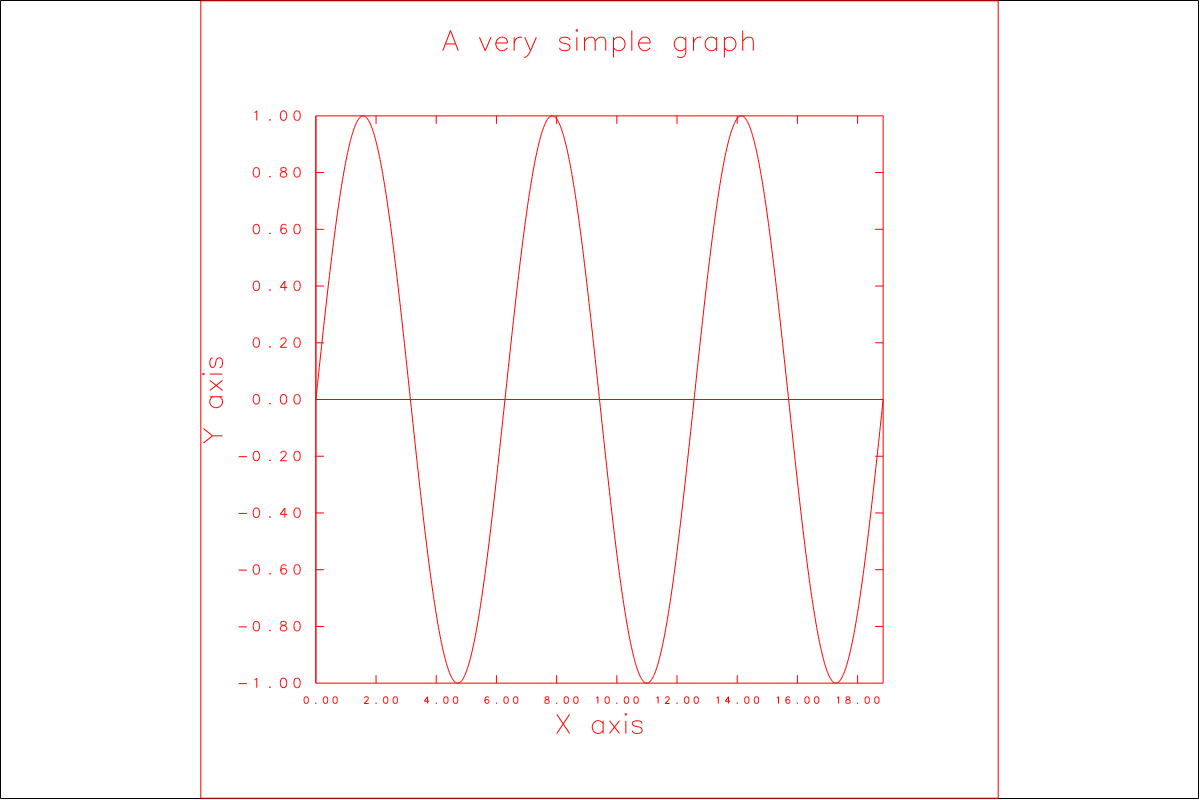
\includegraphics[width=\maxwidth]{../../temp/gr1a001.eps}
  \caption{gr1a001}
  \label{fig:gr1a001}
\end{figure}

\begin{figure}
  \centering
  \includegraphics[width=\maxwidth]{../../temp/gr2001.eps}
  \caption{gr2001}
  \label{fig:gr2001}
\end{figure}

\clearpage
\begin{figure}
  \centering
  \includegraphics[width=\maxwidth]{../../temp/gr3001.eps}
  \caption{gr3001}
  \label{fig:gr3001}
\end{figure}

\begin{figure}
  \centering
  \includegraphics[width=\maxwidth]{../../temp/gr4001.eps}
  \caption{gr4001}
  \label{fig:gr4001}
\end{figure}

\begin{figure}
  \centering
  \includegraphics[width=\maxwidth]{../../temp/gr5001.eps}
  \caption{gr5001}
  \label{fig:gr5001}
\end{figure}

\clearpage
\begin{figure}
  \centering
  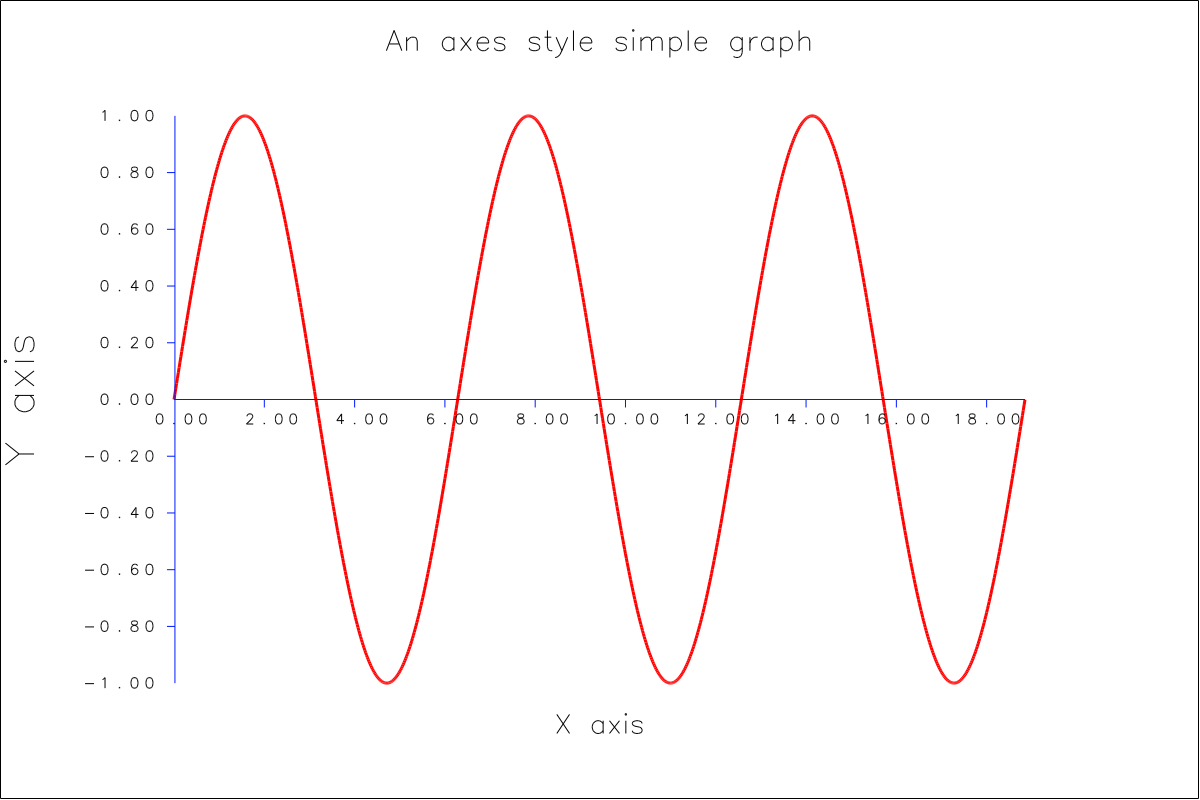
\includegraphics[width=\maxwidth]{../../temp/gr7001.eps}
  \caption{gr7001}
  \label{fig:gr7001}
\end{figure}

\begin{figure}
  \centering
  \includegraphics[width=\maxwidth]{../../temp/gr8001.eps}
  \caption{gr8001}
  \label{fig:gr8001}
\end{figure}

\begin{figure}
  \centering
  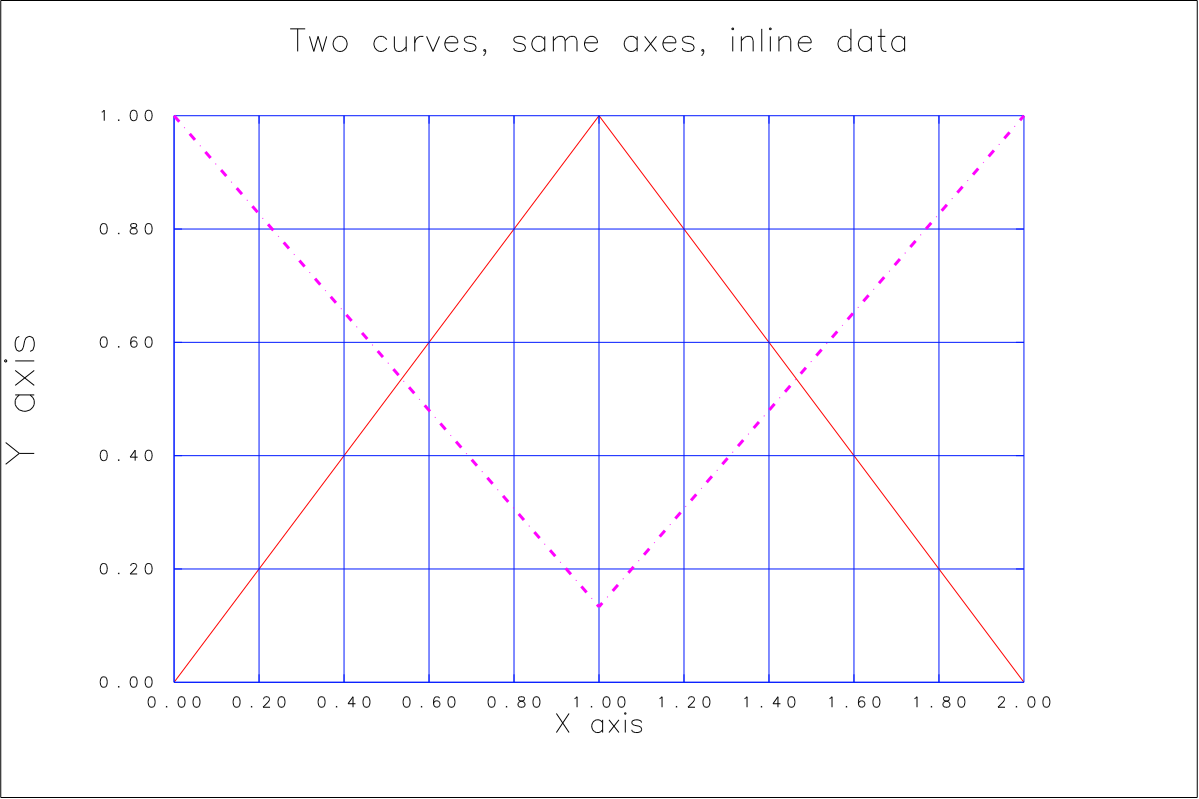
\includegraphics[width=\maxwidth]{../../temp/gr10001.eps}
  \caption{gr10001}
  \label{fig:gr10001}
\end{figure}

\clearpage
\begin{figure}
  \centering
  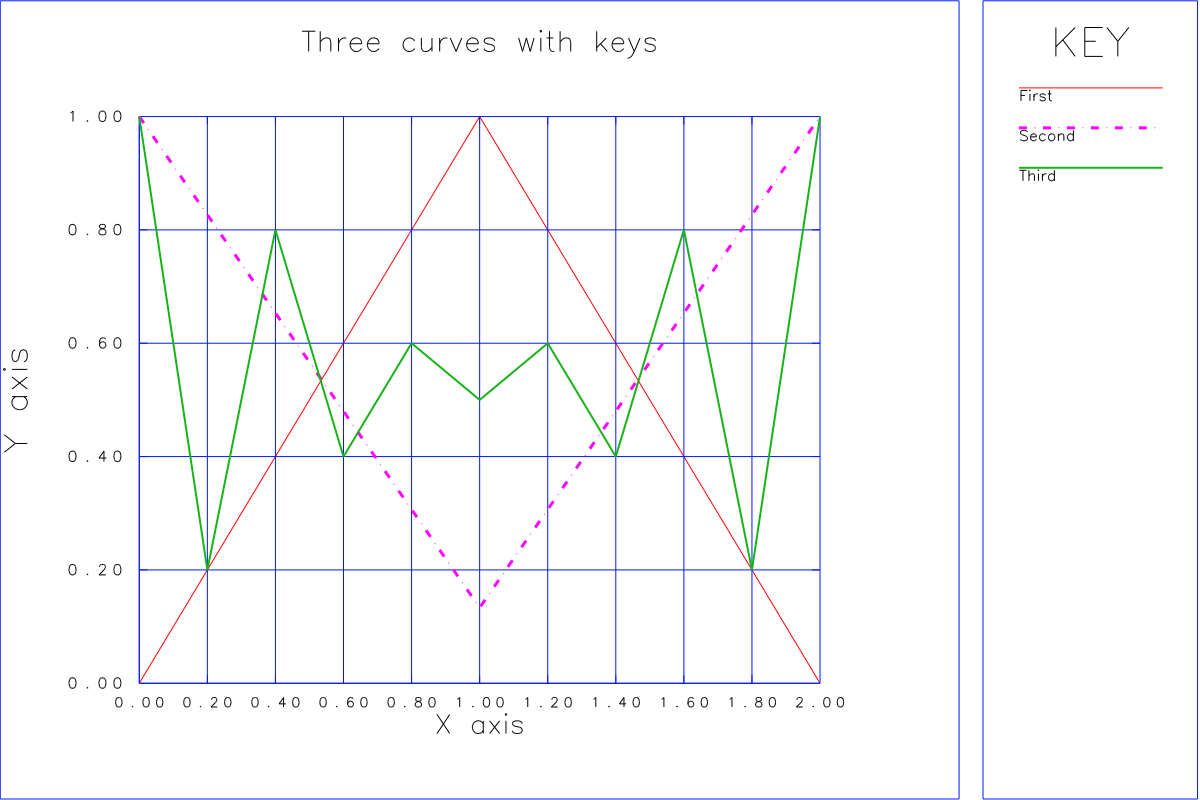
\includegraphics[width=\maxwidth]{../../temp/gr11001.eps}
  \caption{gr11001}
  \label{fig:gr11001}
\end{figure}

\begin{figure}
  \centering
  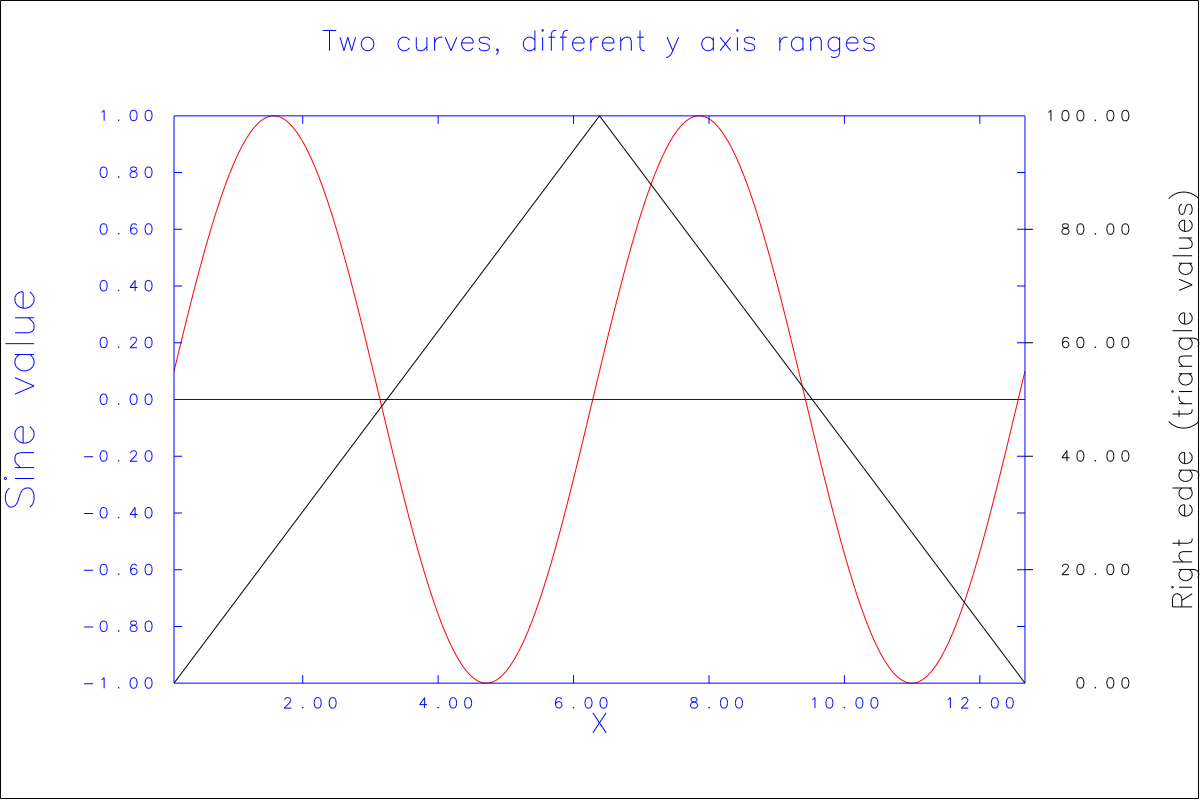
\includegraphics[width=\maxwidth]{../../temp/gr12001.eps}
  \caption{gr12001}
  \label{fig:gr12001}
\end{figure}

\begin{figure}
  \centering
  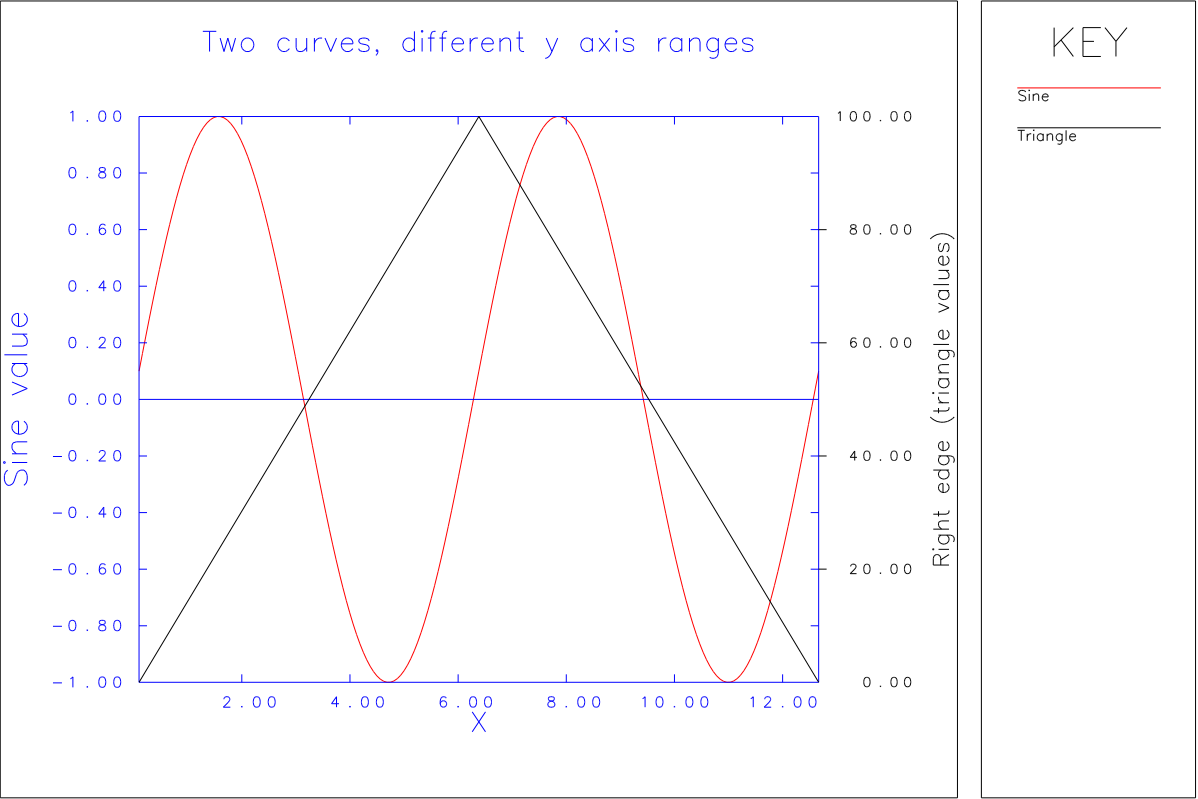
\includegraphics[width=\maxwidth]{../../temp/gr13001.eps}
  \caption{gr13001}
  \label{fig:gr13001}
\end{figure}

\clearpage
\begin{figure}
  \centering
  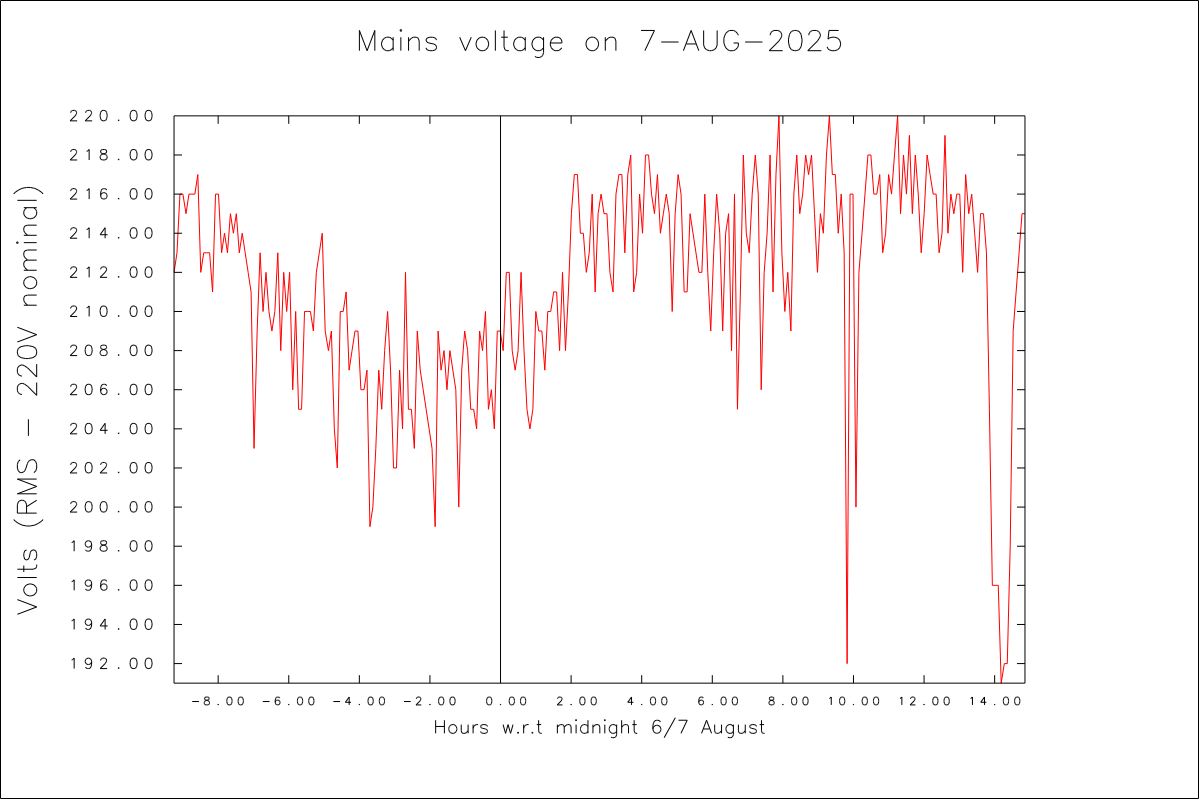
\includegraphics[width=\maxwidth]{../../temp/gr14001.eps}
  \caption{gr14001}
  \label{fig:gr14001}
\end{figure}

\begin{figure}
  \centering
  \includegraphics[width=\maxwidth]{../../temp/gr15001.eps}
  \caption{gr15001}
  \label{fig:gr15001}
\end{figure}

\begin{figure}
  \centering
  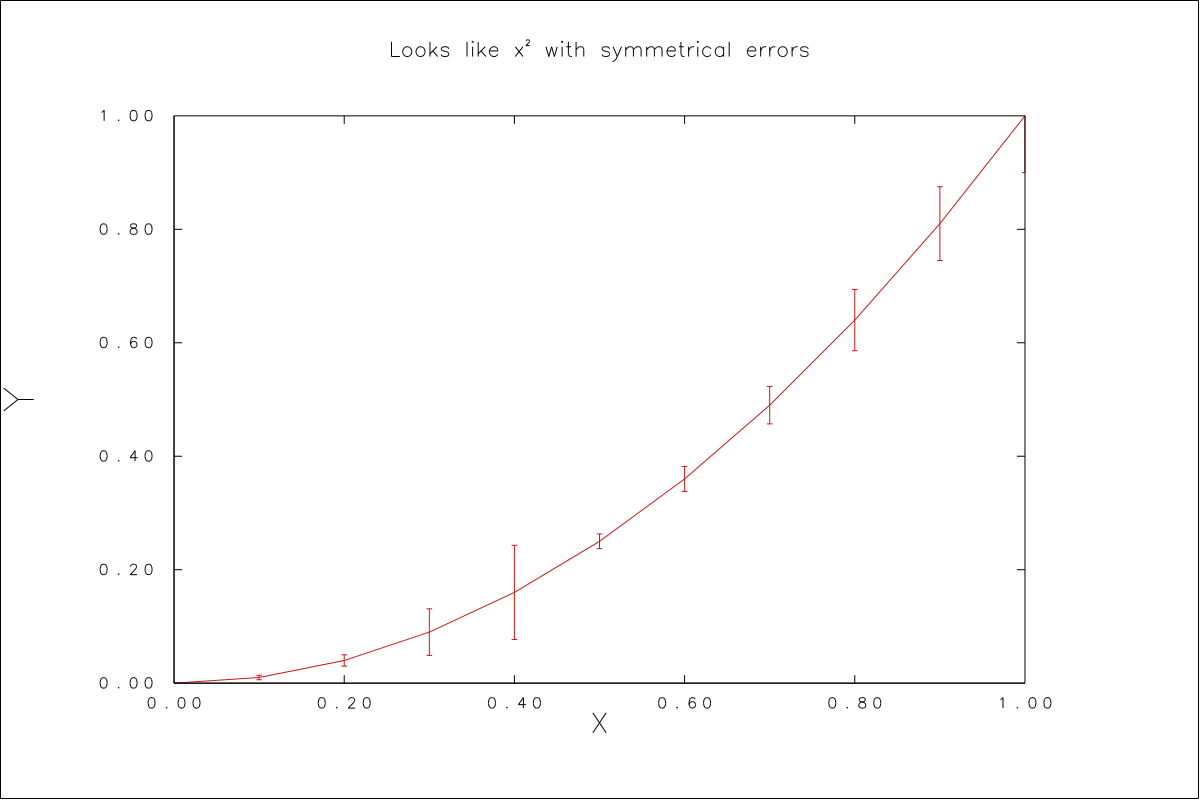
\includegraphics[width=\maxwidth]{../../temp/gr16001.eps}
  \caption{gr16001}
  \label{fig:gr16001}
\end{figure}

\clearpage
\begin{figure}
  \centering
  \includegraphics[width=\maxwidth]{../../temp/gr17001.eps}
  \caption{gr17001}
  \label{fig:gr17001}
\end{figure}

\begin{figure}
  \centering
  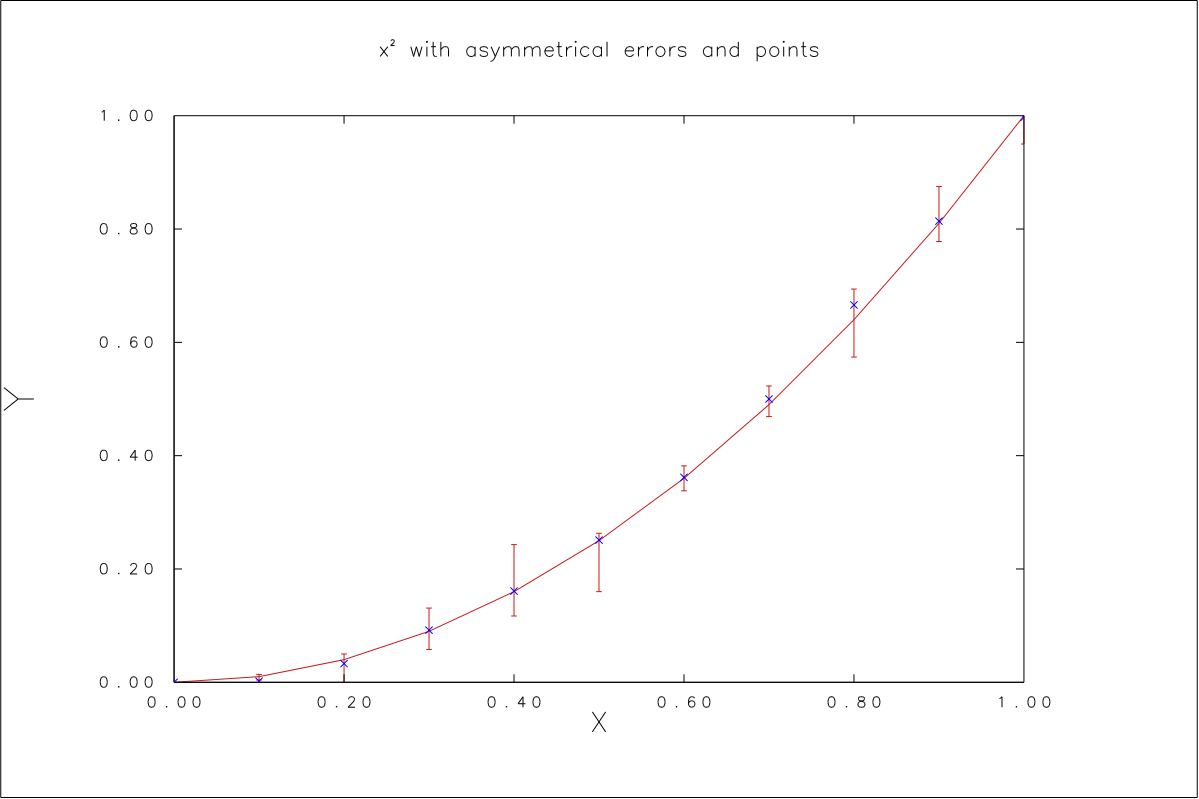
\includegraphics[width=\maxwidth]{../../temp/gr18001.eps}
  \caption{gr18001}
  \label{fig:gr18001}
\end{figure}

\begin{figure}
  \centering
  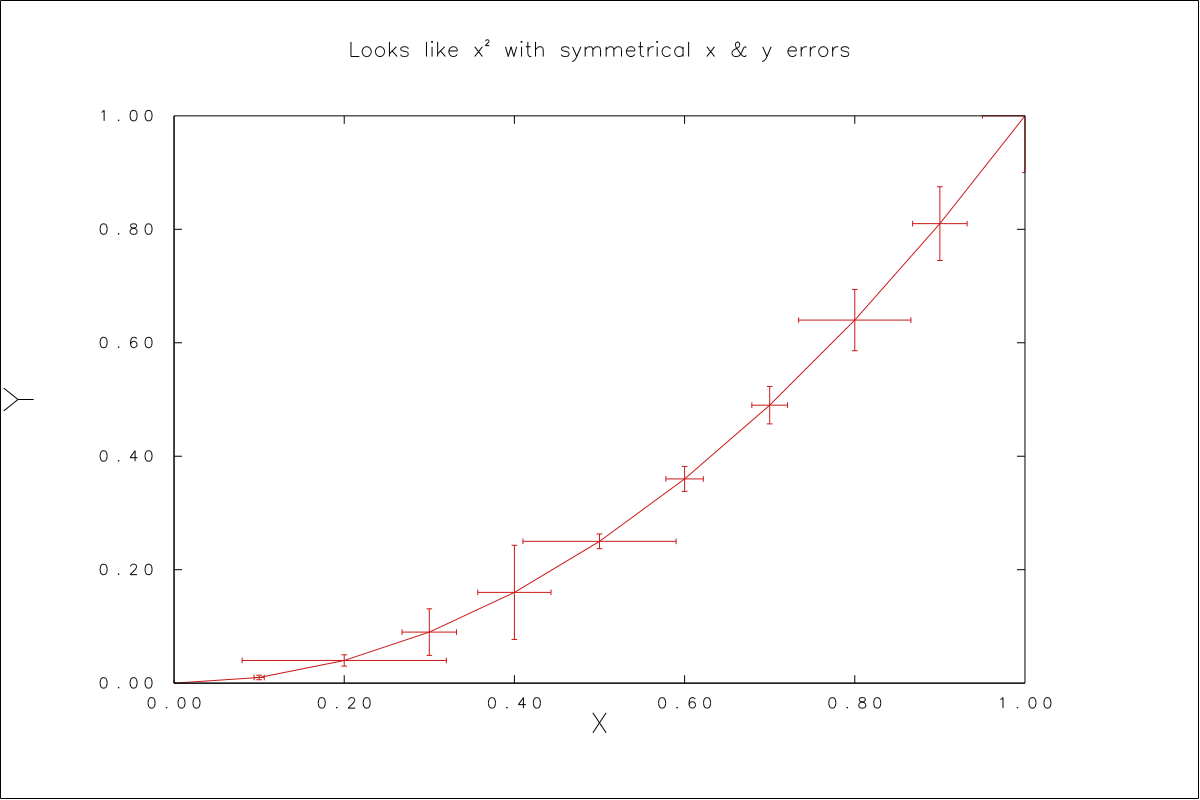
\includegraphics[width=\maxwidth]{../../temp/gr1x001.eps}
  \caption{gr1x001}
  \label{fig:gr1x001}
\end{figure}

\clearpage
\begin{figure}
  \centering
  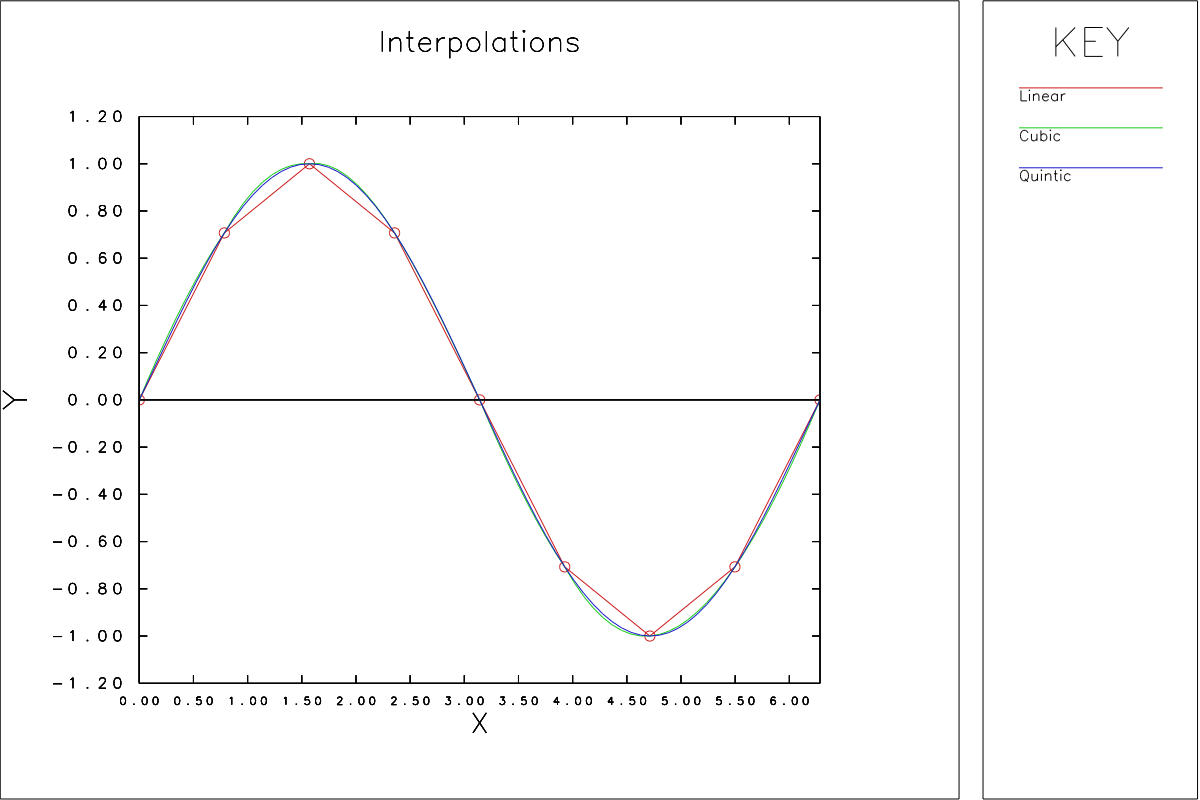
\includegraphics[width=\maxwidth]{../../temp/gr1i001.eps}
  \caption{gr1i001}
  \label{fig:gr1i001}
\end{figure}

\begin{figure}
  \centering
  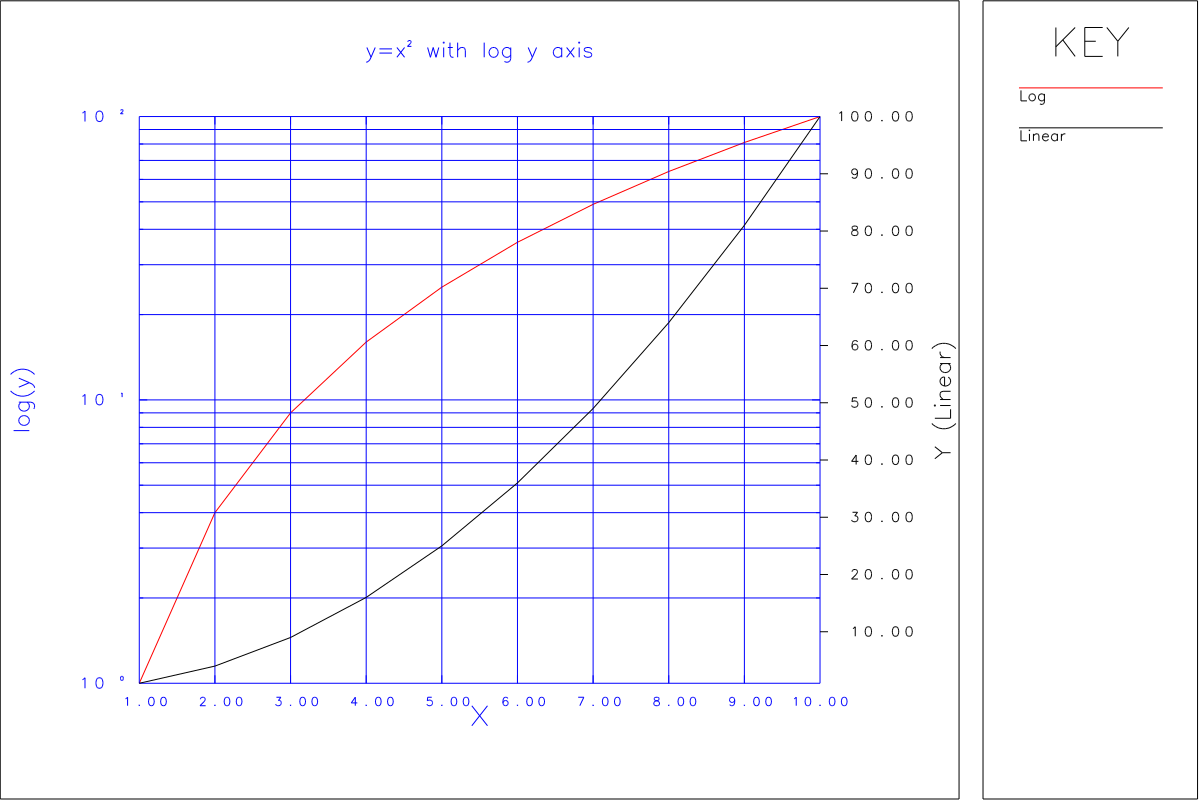
\includegraphics[width=\maxwidth]{../../temp/gr20001.eps}
  \caption{gr20001}
  \label{fig:gr20001}
\end{figure}

\begin{figure}
  \centering
  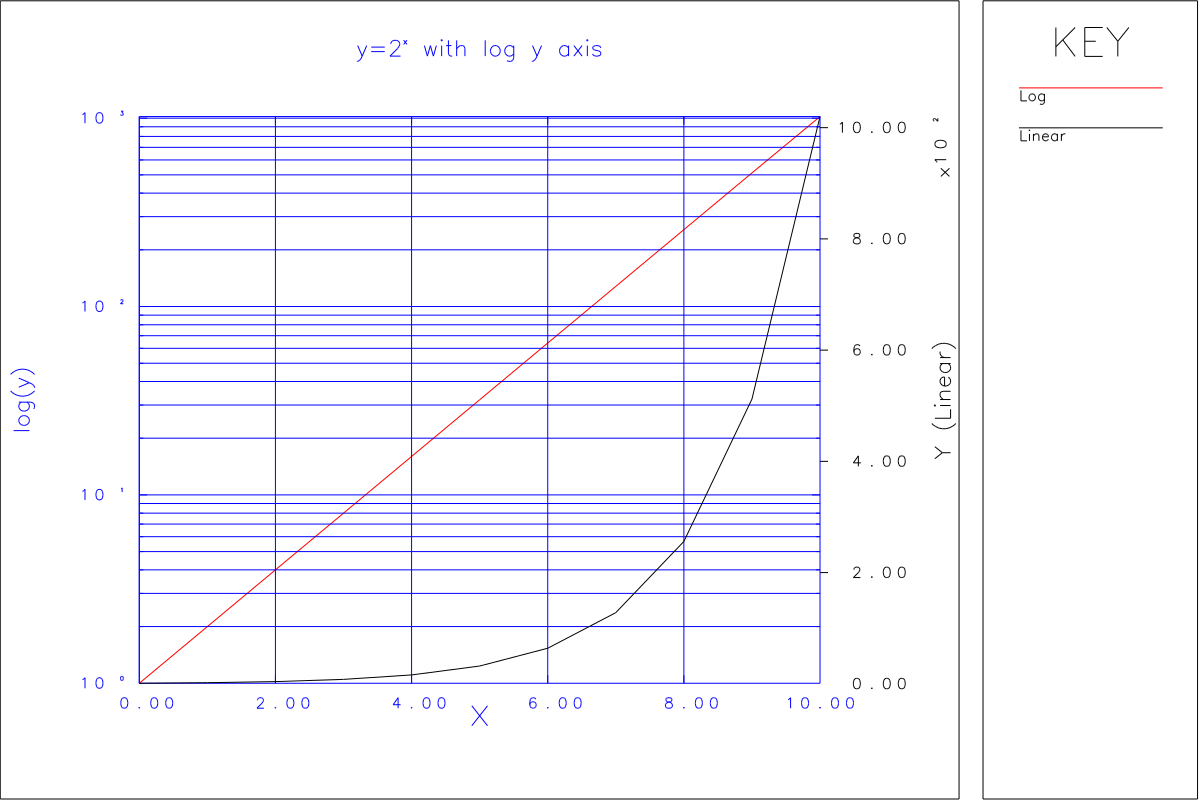
\includegraphics[width=\maxwidth]{../../temp/gr2a001.eps}
  \caption{gr2a001}
  \label{fig:gr2a001}
\end{figure}

\clearpage
\begin{figure}
  \centering
  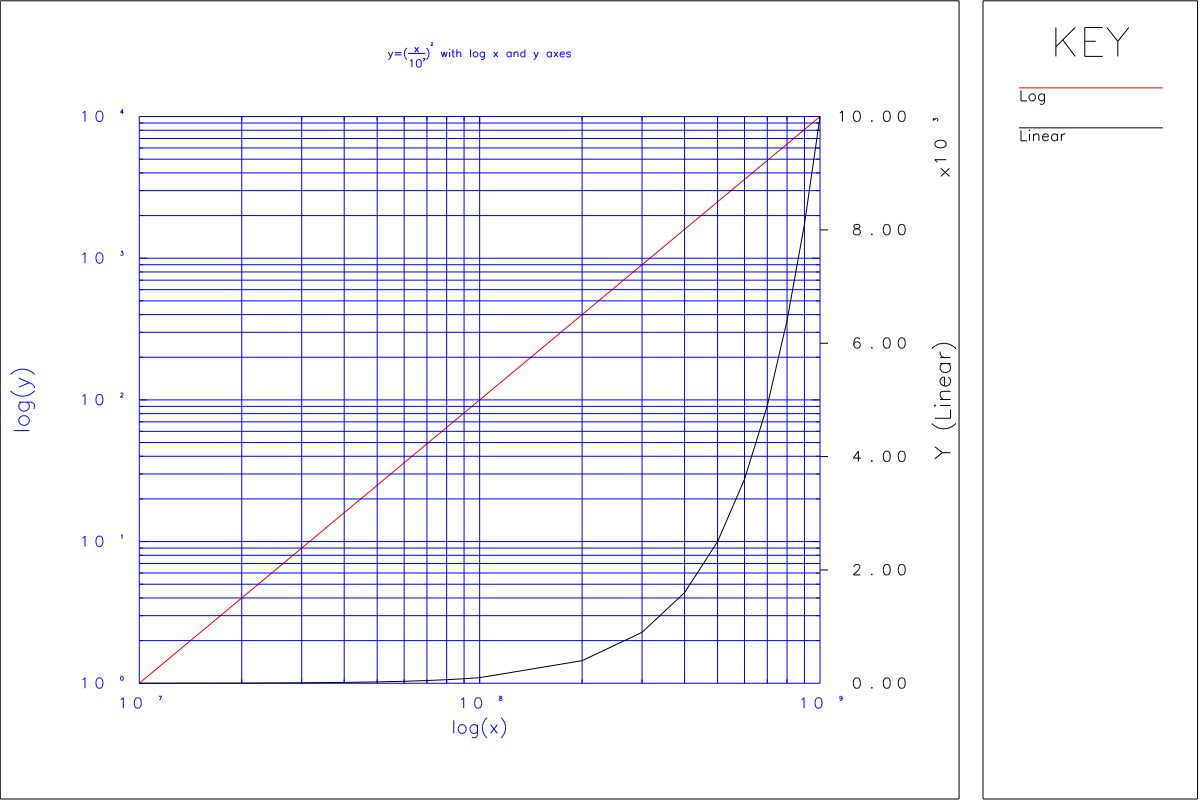
\includegraphics[width=\maxwidth]{../../temp/gr21001.eps}
  \caption{gr21001}
  \label{fig:gr21001}
\end{figure}

\begin{figure}
  \centering
  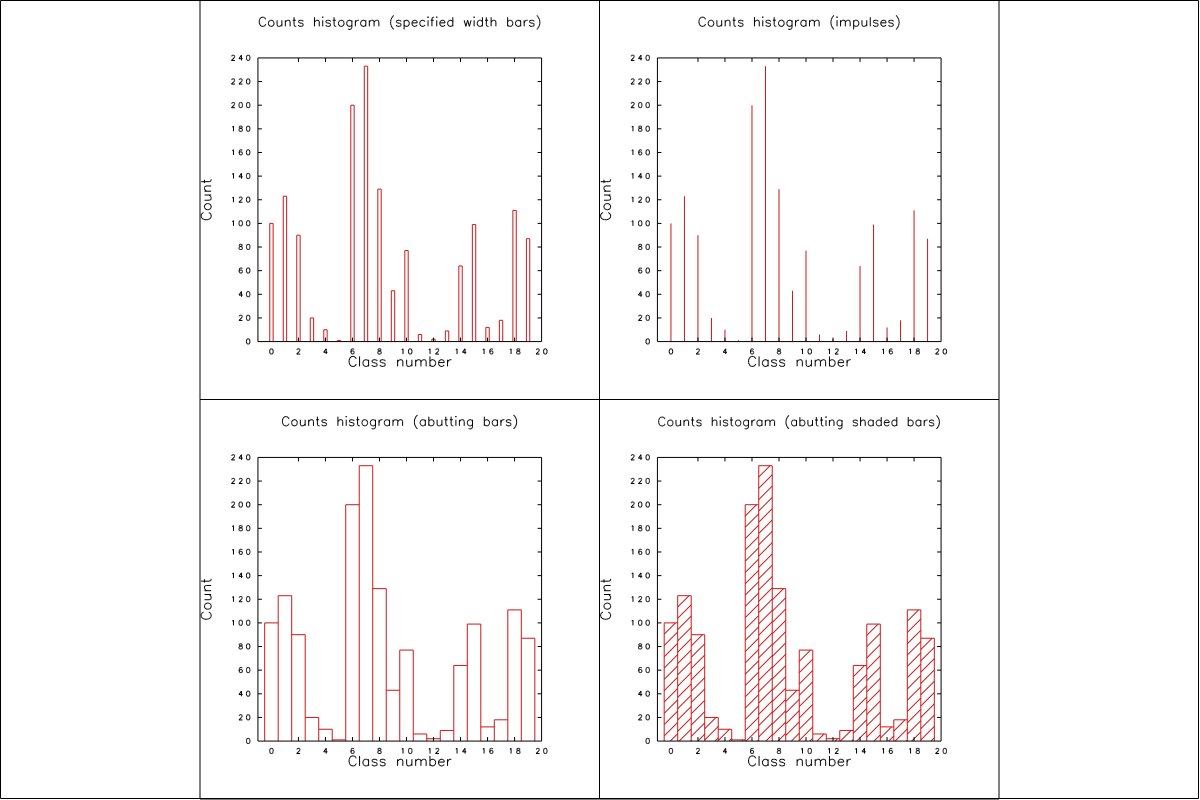
\includegraphics[width=\maxwidth]{../../temp/gr22001.eps}
  \caption{gr22001}
  \label{fig:gr22001}
\end{figure}

\begin{figure}
  \centering
  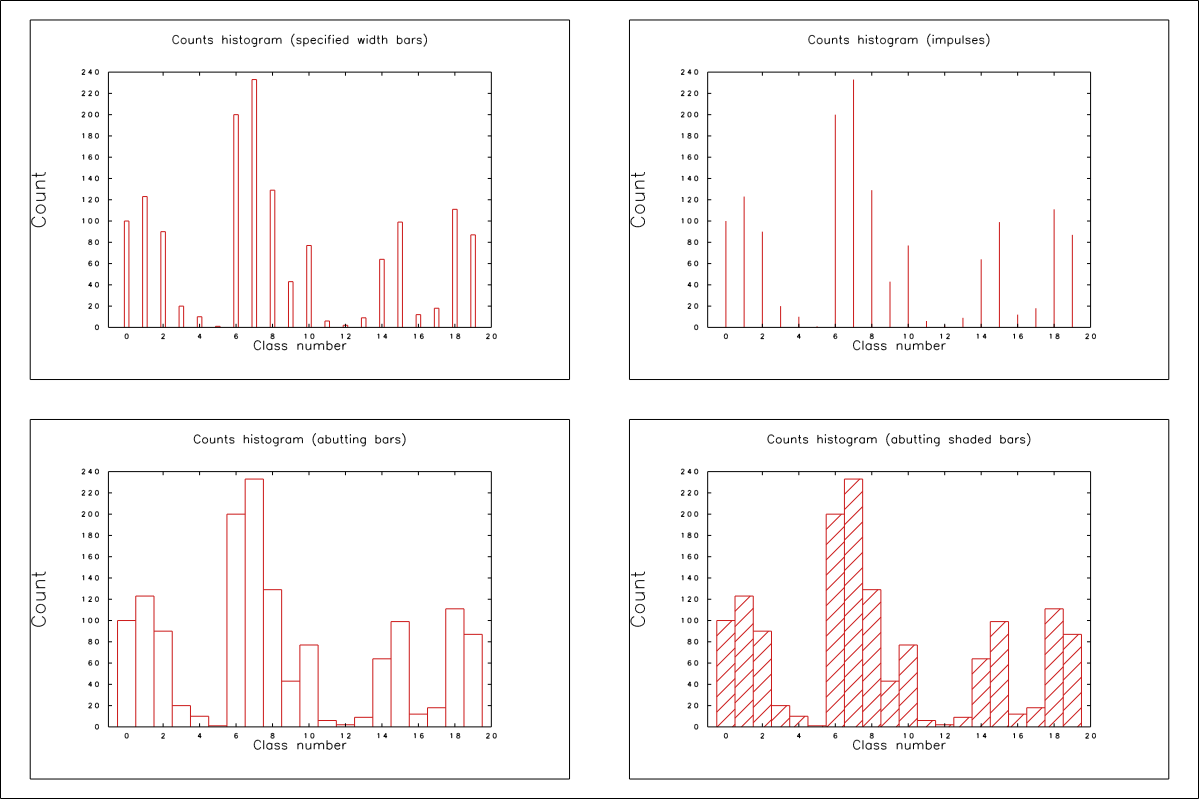
\includegraphics[width=\maxwidth]{../../temp/gr29001.eps}
  \caption{gr29001}
  \label{fig:gr29001}
\end{figure}

\clearpage
\begin{figure}
  \centering
  \includegraphics[width=\maxwidth]{../../temp/gr28001.eps}
  \caption{gr28001}
  \label{fig:gr28001}
\end{figure}

\begin{figure}
  \centering
  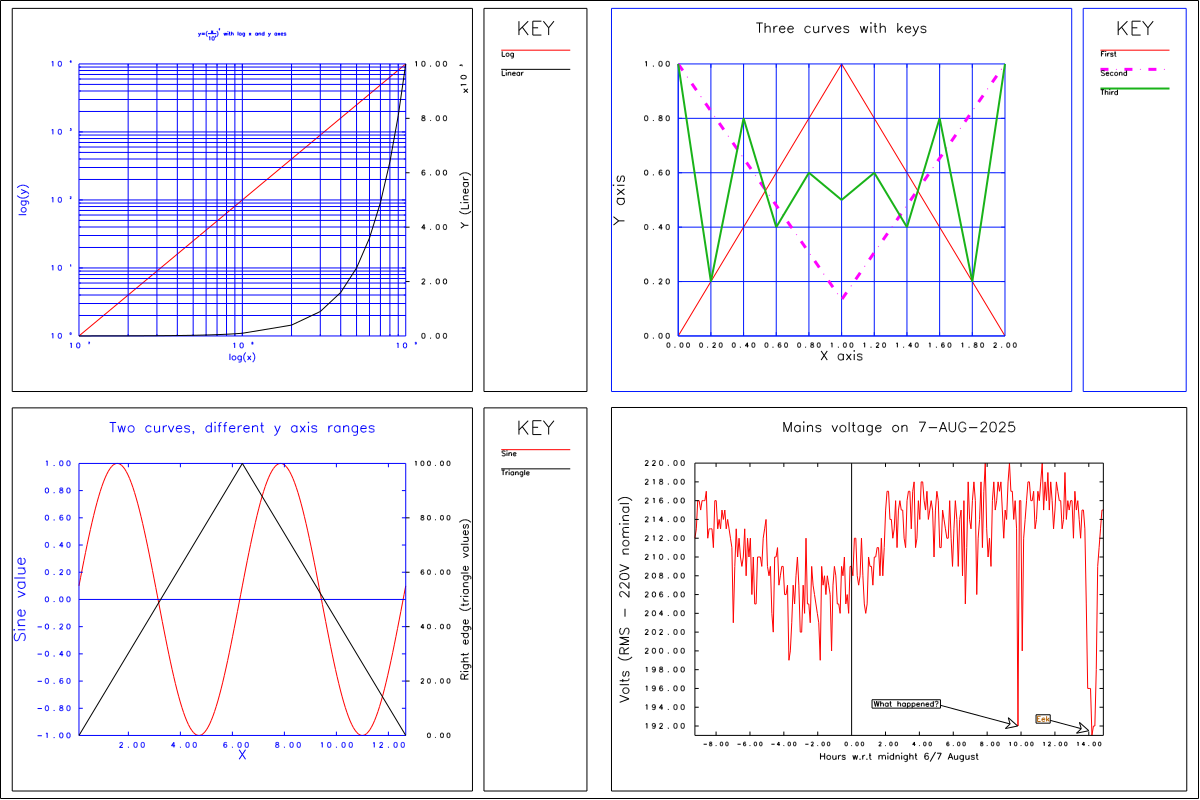
\includegraphics[width=\maxwidth]{../../temp/gr27001.eps}
  \caption{gr27001}
  \label{fig:gr27001}
\end{figure}

\begin{figure}
  \centering
  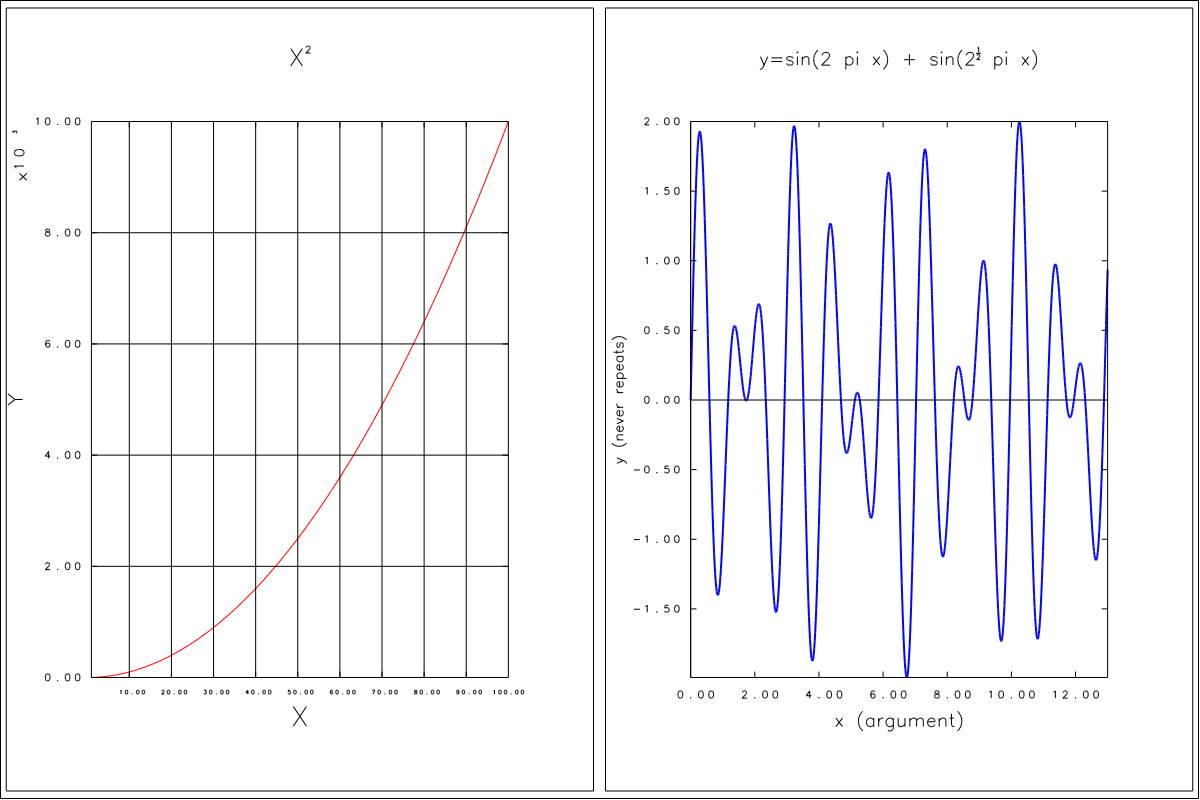
\includegraphics[width=\maxwidth]{../../temp/gr30001.eps}
  \caption{gr30001}
  \label{fig:gr30001}
\end{figure}

\clearpage
\begin{figure}
  \centering
  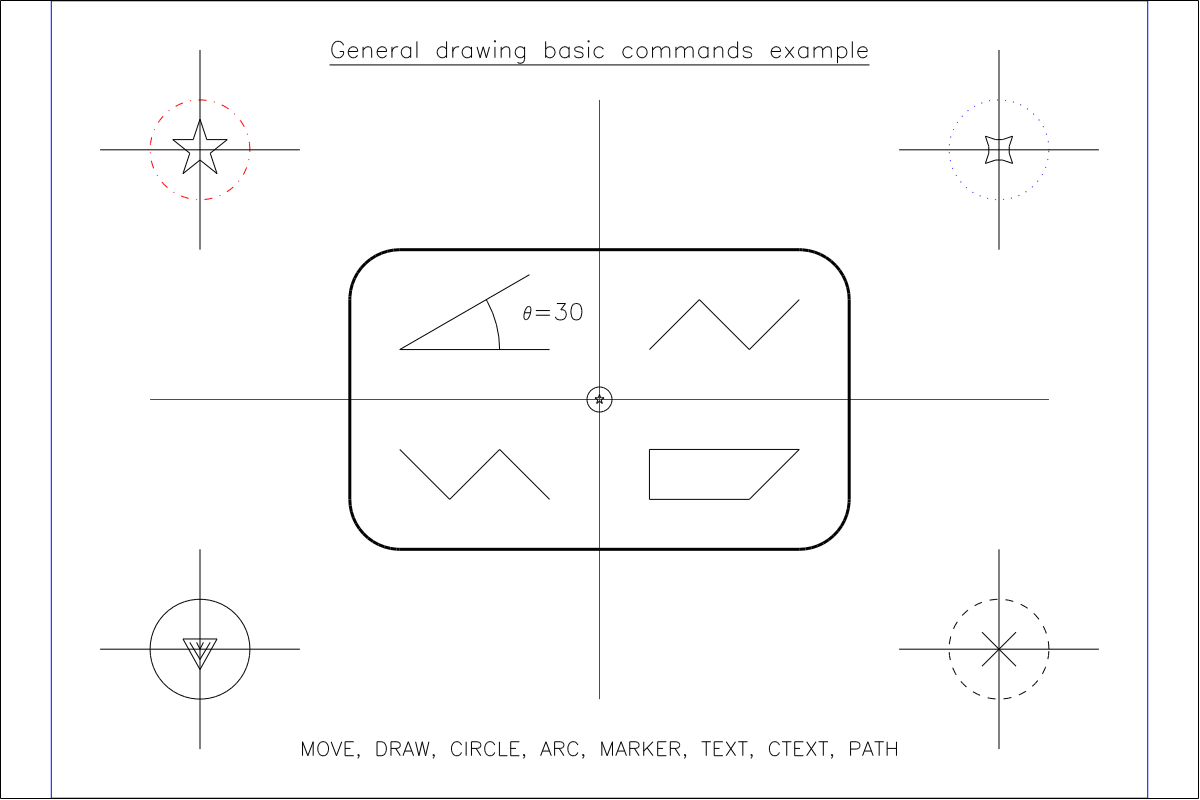
\includegraphics[width=\maxwidth]{../../temp/gd01001.eps}
  \caption{gd01001}
  \label{fig:gd01001}
\end{figure}

\begin{figure}
  \centering
  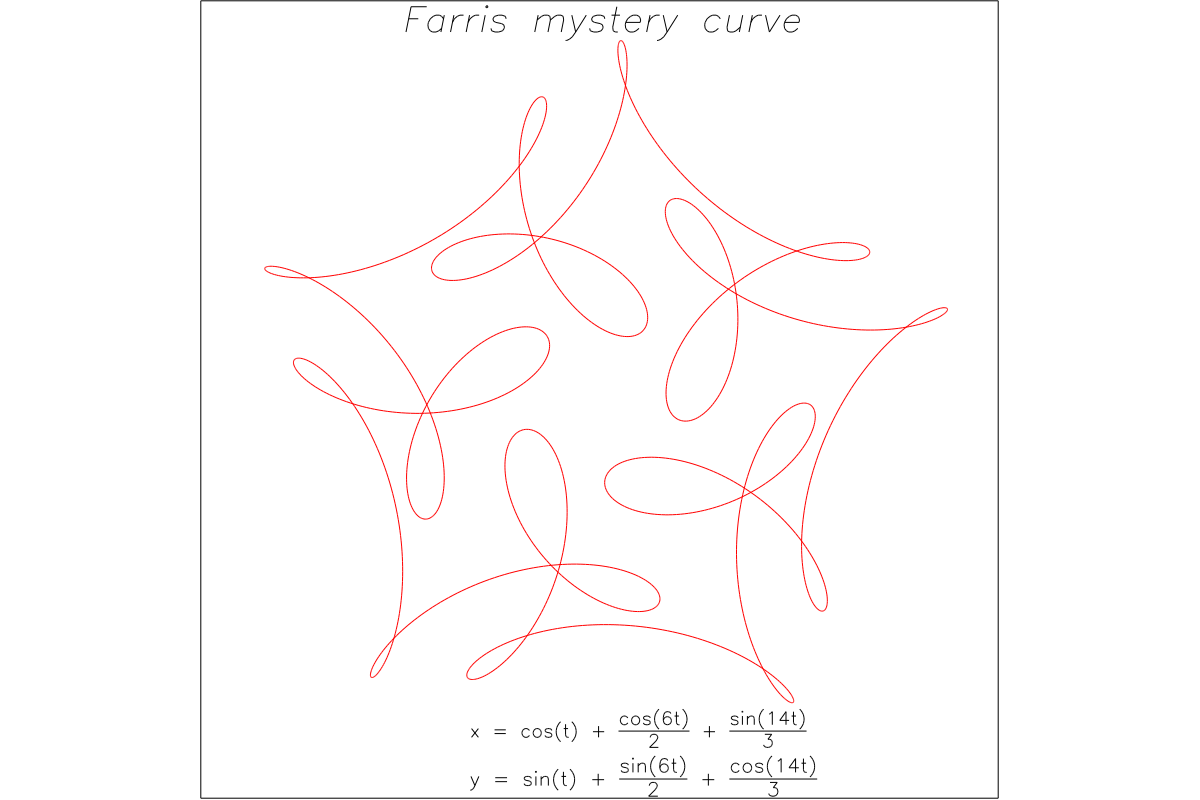
\includegraphics[width=\maxwidth]{../../temp/g1fm001.eps}
  \caption{g1fm001}
  \label{fig:g1fm001}
\end{figure}

\begin{figure}
  \centering
  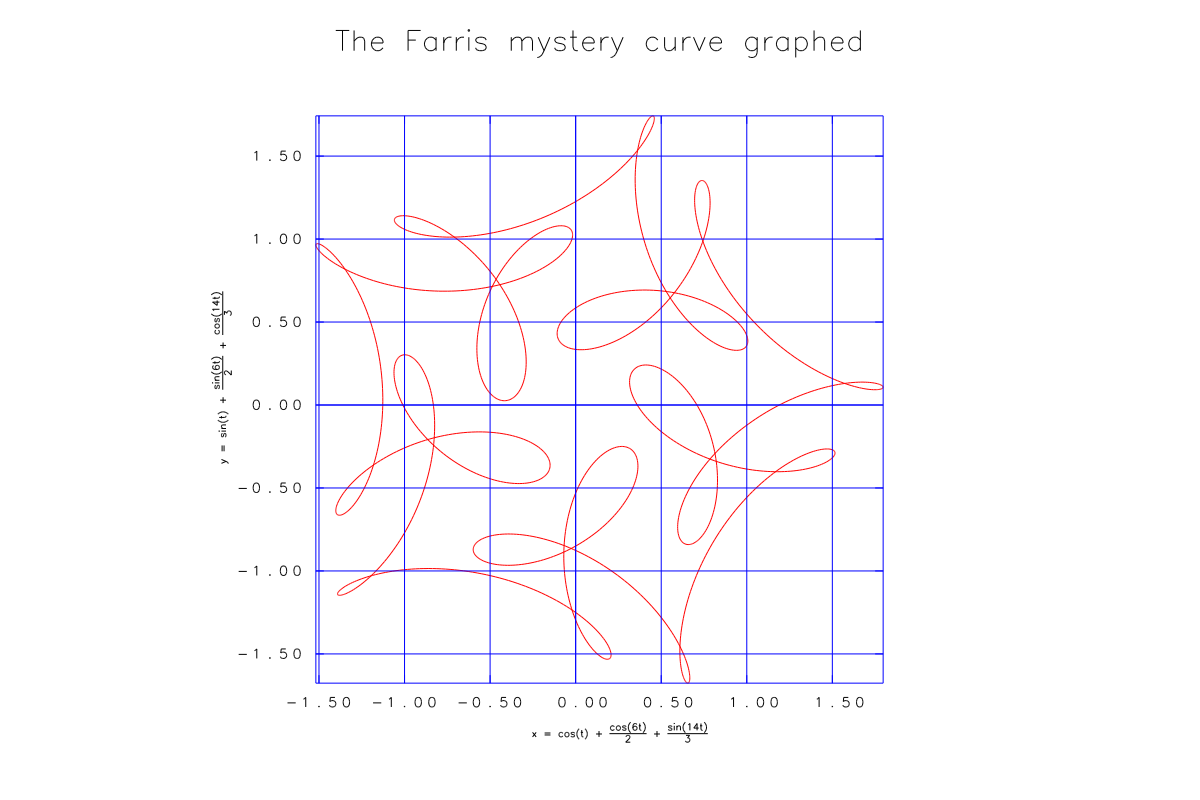
\includegraphics[width=\maxwidth]{../../temp/g2fm001.eps}
  \caption{g2fm001}
  \label{fig:g2fm001}
\end{figure}

\clearpage
\begin{figure}
  \centering
  
\includegraphics[width=\maxwidth]{../../temp/g1sp001.eps}
  \caption{g1sp001}
  \label{fig:g1sp001}
\end{figure}

\begin{figure}
  \centering
  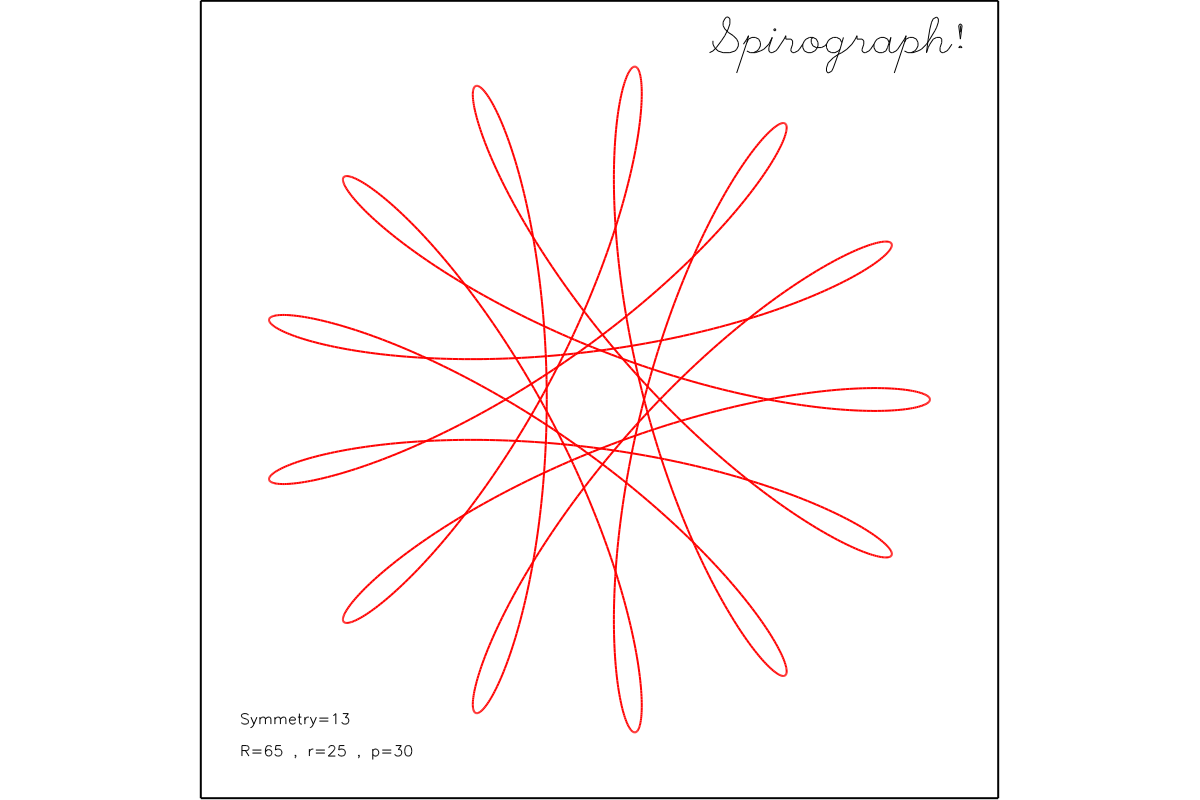
\includegraphics[width=\maxwidth]{../../temp/g2sp001.eps}
  \caption{g2sp001}
  \label{fig:g2sp001}
\end{figure}

\begin{figure}
  \centering
  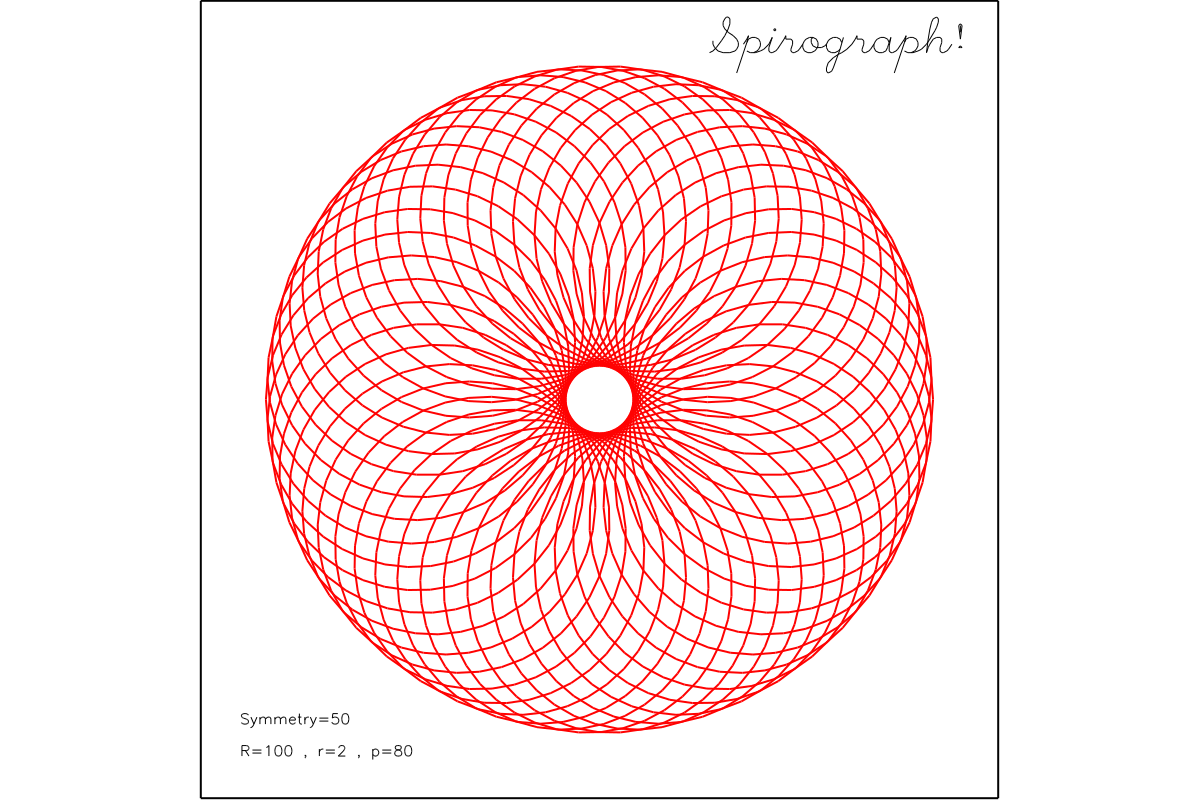
\includegraphics[width=\maxwidth]{../../temp/g3sp001.eps}
  \caption{g3sp001}
  \label{fig:g3sp001}
\end{figure}

\clearpage
\begin{figure}
  \centering
  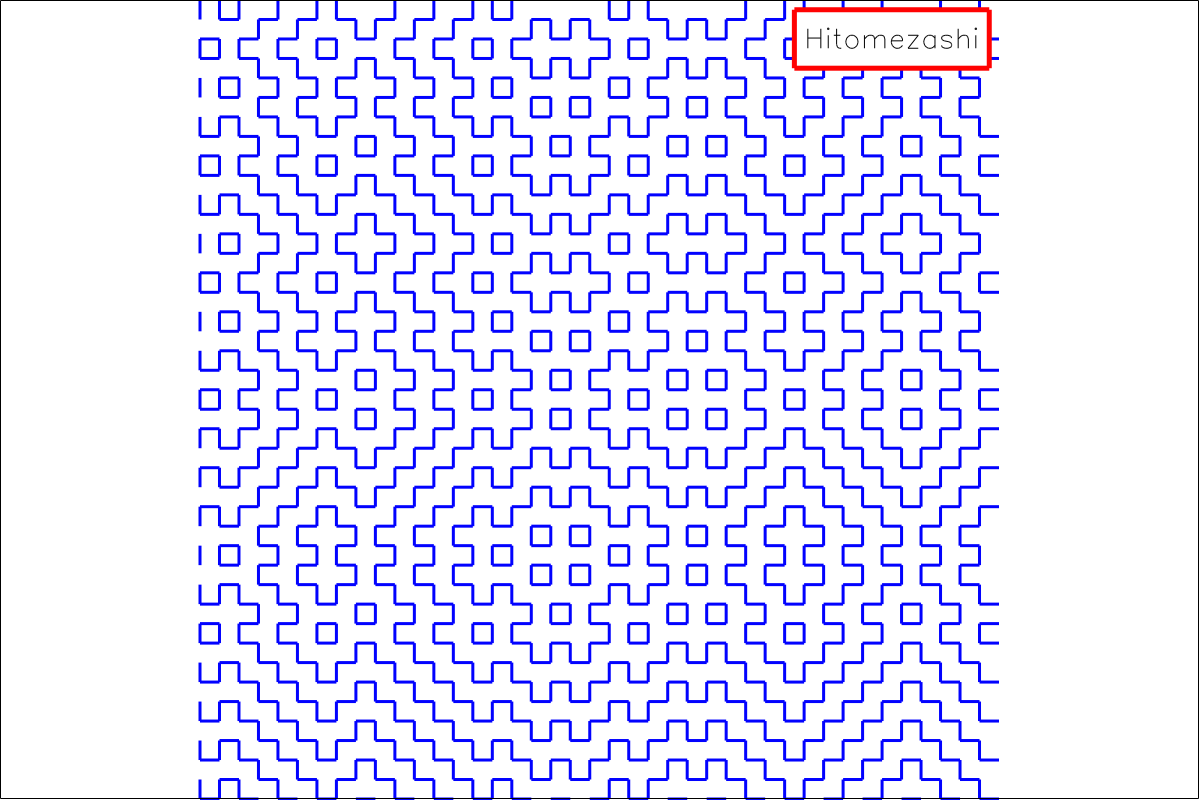
\includegraphics[width=\maxwidth]{../../temp/gemz001.eps}
  \caption{gemz001}
  \label{fig:gemz001}
\end{figure}

\begin{figure}
  \centering
  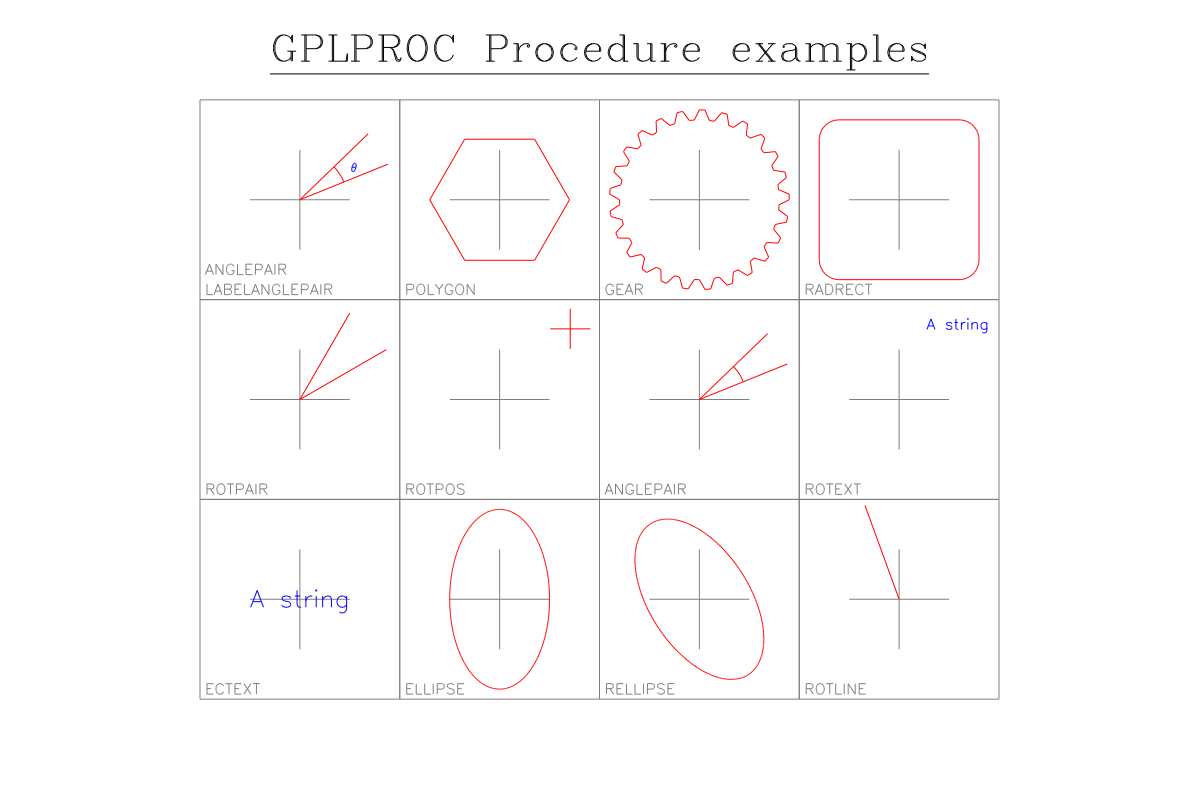
\includegraphics[width=\maxwidth]{../../temp/gdea001.eps}
  \caption{gdea001}
  \label{fig:gdea001}
\end{figure}

\begin{figure}
  \centering
  
\includegraphics[width=\maxwidth]{../../temp/gh1b001.eps}
  \caption{gh1b001}
  \label{fig:gh1b001}
\end{figure}

\clearpage
\begin{figure}
  \centering
  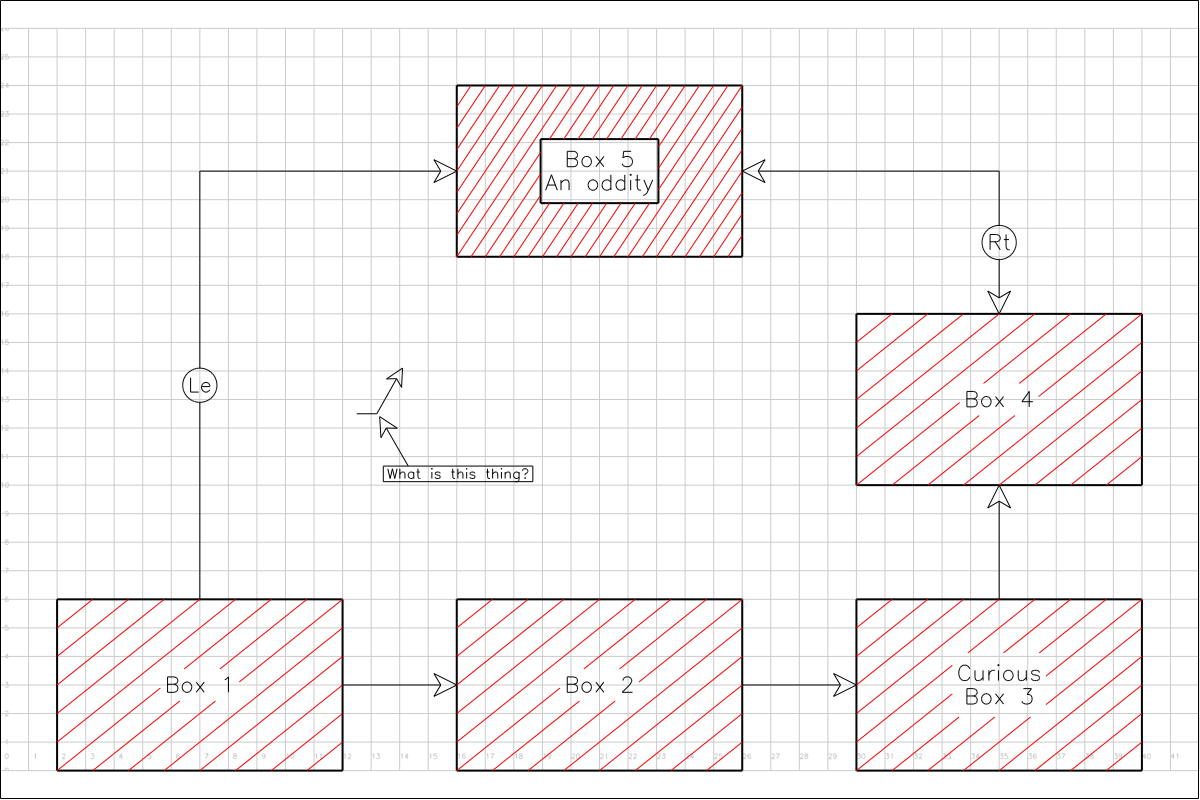
\includegraphics[width=\maxwidth]{../../temp/ghbb001.eps}
  \caption{ghbb001}
  \label{fig:ghbb001}
\end{figure}

\begin{figure}
  \centering
  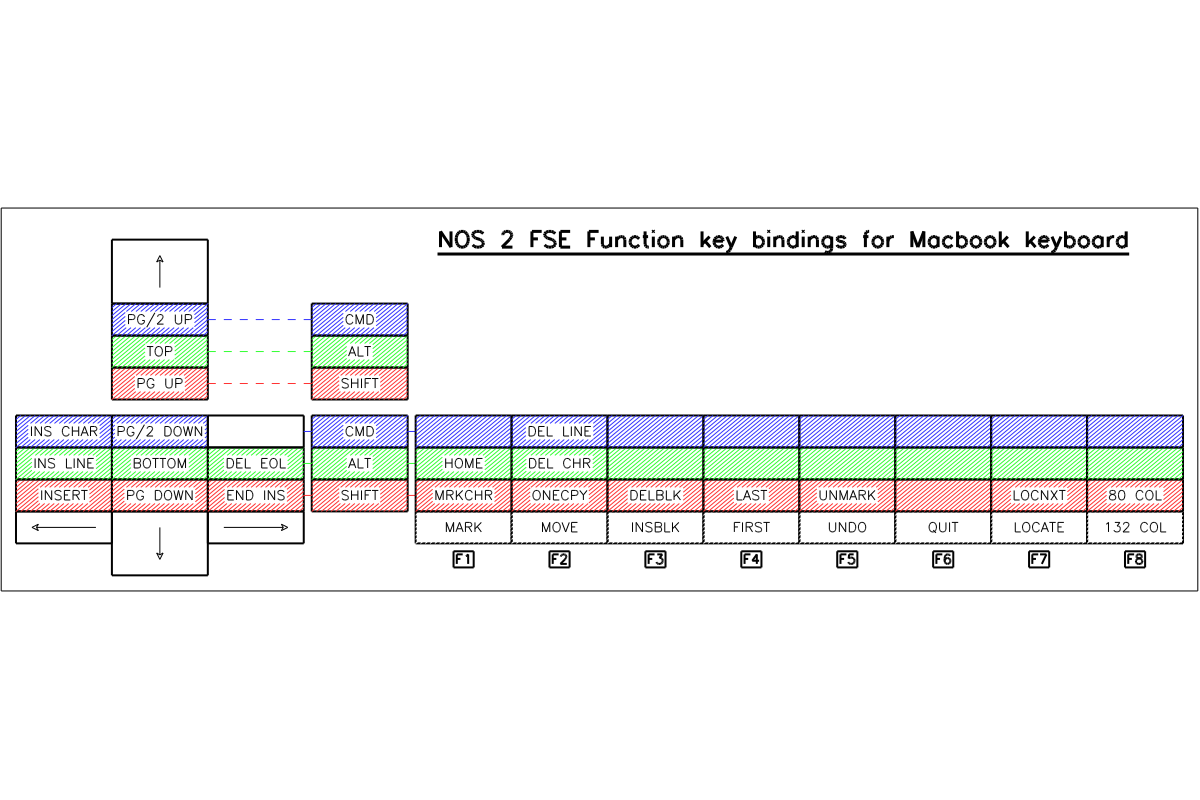
\includegraphics[width=\maxwidth]{../../temp/gh2b001.eps}
  \caption{gh2b001}
  \label{fig:gh2b001}
\end{figure}

\begin{figure}
  \centering
  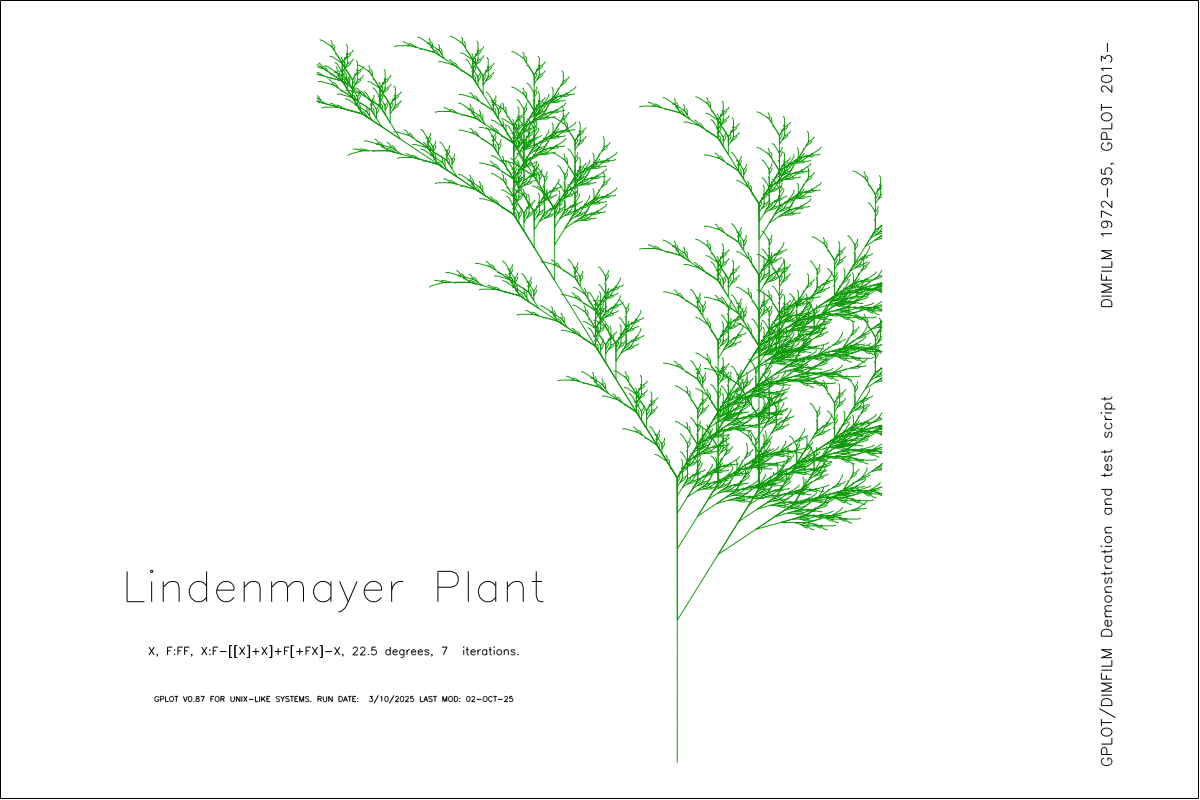
\includegraphics[width=\maxwidth]{../../temp/lsys001.eps}
  \caption{lsys001}
  \label{fig:lsys001}
\end{figure}

\clearpage
\begin{figure}
  \centering
  
\includegraphics[width=\maxwidth]{../../temp/fosm001.eps}
  \caption{fosm001}
  \label{fig:fosm001}
\end{figure}

\begin{figure}
  \centering
  \includegraphics[width=\maxwidth]{../../temp/cht1001.eps}
  \caption{cht1001}
  \label{fig:cht1001}
\end{figure}

\begin{figure}
  \centering
  \includegraphics[width=\maxwidth]{../../temp/cht2001.eps}
  \caption{cht2001}
  \label{fig:cht2001}
\end{figure}

\clearpage
\begin{figure}
  \centering
  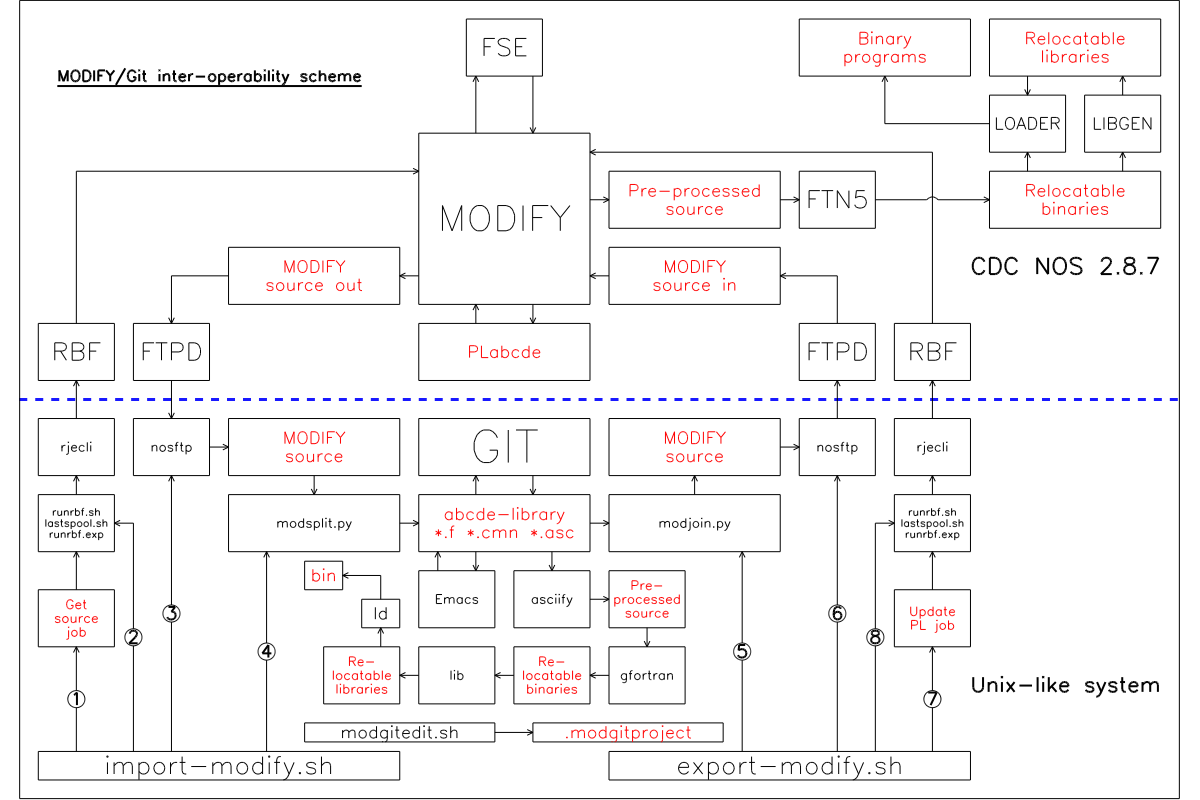
\includegraphics[width=\maxwidth]{../../temp/iocd001.eps}
  \caption{iocd001}
  \label{fig:iocd001}
\end{figure}

\begin{figure}
  \centering
  \includegraphics[width=\maxwidth]{../../temp/f01t001.eps}
  \caption{f01t001}
  \label{fig:f01t001}
\end{figure}

\begin{figure}
  \centering
  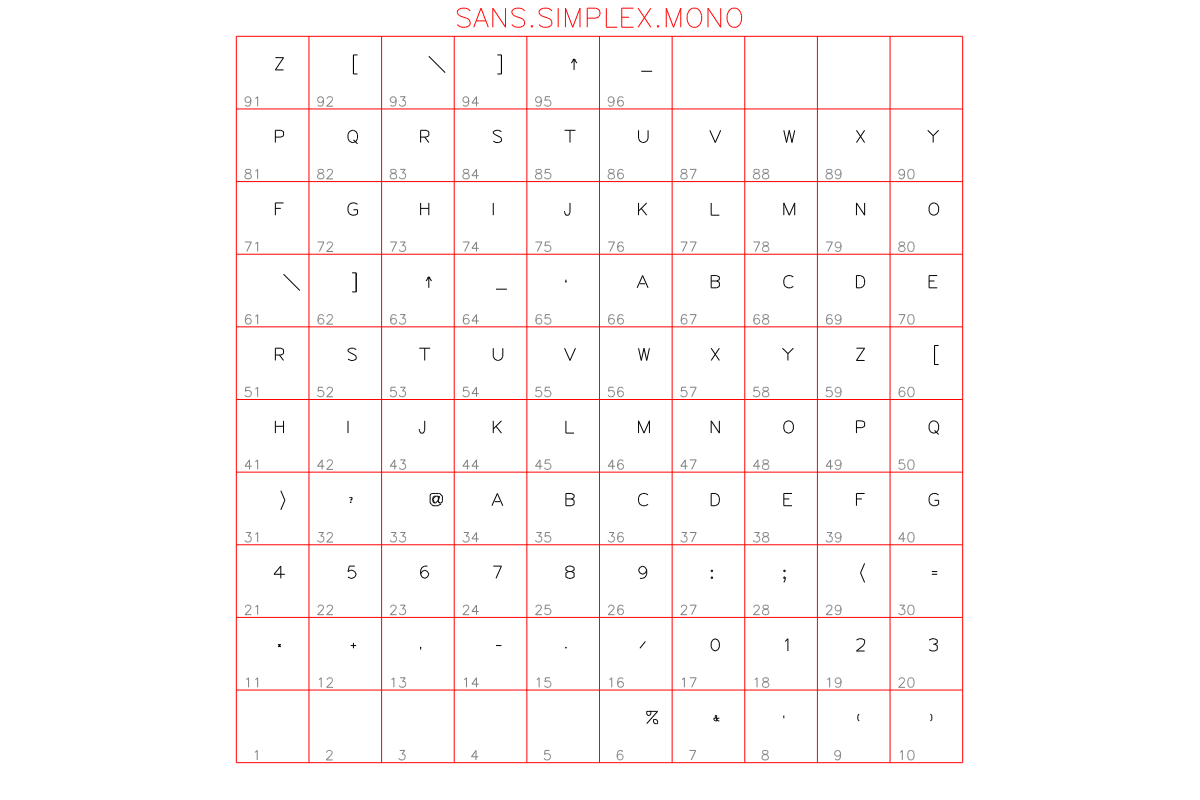
\includegraphics[width=\maxwidth]{../../temp/f02t001.eps}
  \caption{f02t001}
  \label{fig:f02t001}
\end{figure}

\clearpage
\begin{figure}
  \centering
  \includegraphics[width=\maxwidth]{../../temp/f03t001.eps}
  \caption{f03t001}
  \label{fig:f03t001}
\end{figure}

\begin{figure}
  \centering
  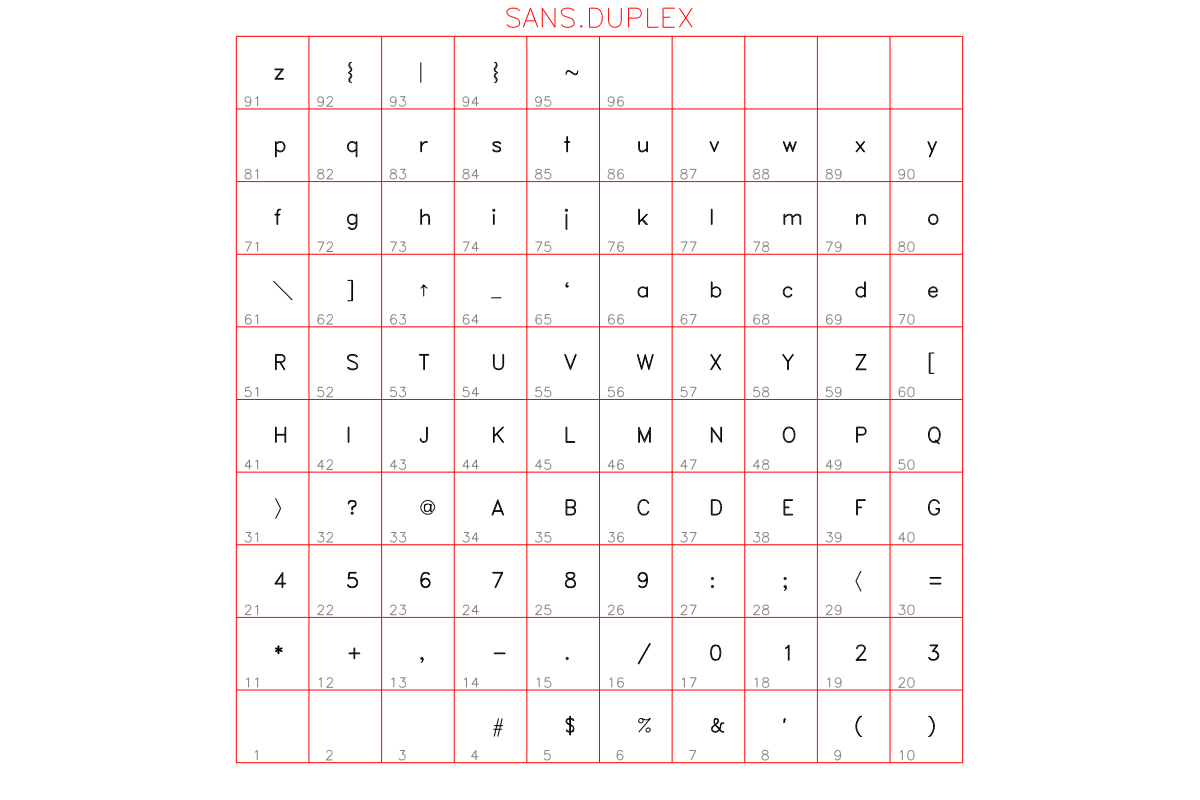
\includegraphics[width=\maxwidth]{../../temp/f04t001.eps}
  \caption{f04t001}
  \label{fig:f04t001}
\end{figure}

\begin{figure}
  \centering
  \includegraphics[width=\maxwidth]{../../temp/f05t001.eps}
  \caption{f05t001}
  \label{fig:f05t001}
\end{figure}

\clearpage
\begin{figure}
  \centering
  \includegraphics[width=\maxwidth]{../../temp/f06t001.eps}
  \caption{f06t001}
  \label{fig:f06t001}
\end{figure}

\begin{figure}
  \centering
  \includegraphics[width=\maxwidth]{../../temp/f07t001.eps}
  \caption{f07t001}
  \label{fig:f07t001}
\end{figure}

\begin{figure}
  \centering
  \includegraphics[width=\maxwidth]{../../temp/f08t001.eps}
  \caption{f08t001}
  \label{fig:f08t001}
\end{figure}

\clearpage
\begin{figure}
  \centering
  \includegraphics[width=\maxwidth]{../../temp/f09t001.eps}
  \caption{f09t001}
  \label{fig:f09t001}
\end{figure}

\begin{figure}
  \centering
  \includegraphics[width=\maxwidth]{../../temp/f10t001.eps}
  \caption{f10t001}
  \label{fig:f10t001}
\end{figure}

\begin{figure}
  \centering
  \includegraphics[width=\maxwidth]{../../temp/f11t001.eps}
  \caption{f11t001}
  \label{fig:f11t001}
\end{figure}

\clearpage
\begin{figure}
  \centering
  \includegraphics[width=\maxwidth]{../../temp/f12t001.eps}
  \caption{f12t001}
  \label{fig:f12t001}
\end{figure}

\begin{figure}
  \centering
  \includegraphics[width=\maxwidth]{../../temp/f13t001.eps}
  \caption{f13t001}
  \label{fig:f13t001}
\end{figure}

\begin{figure}
  \centering
  \includegraphics[width=\maxwidth]{../../temp/f14t001.eps}
  \caption{f14t001}
  \label{fig:f14t001}
\end{figure}

\clearpage
\begin{figure}
  \centering
  \includegraphics[width=\maxwidth]{../../temp/f15t001.eps}
  \caption{f15t001}
  \label{fig:f15t001}
\end{figure}

\begin{figure}
  \centering
  \includegraphics[width=\maxwidth]{../../temp/f16t001.eps}
  \caption{f16t001}
  \label{fig:f16t001}
\end{figure}

\begin{figure}
  \centering
  \includegraphics[width=\maxwidth]{../../temp/f17t001.eps}
  \caption{f17t001}
  \label{fig:f17t001}
\end{figure}

\clearpage
\begin{figure}
  \centering
  \includegraphics[width=\maxwidth]{../../temp/f18t001.eps}
  \caption{f18t001}
  \label{fig:f18t001}
\end{figure}

\begin{figure}
  \centering
  \includegraphics[width=\maxwidth]{../../temp/f01s001.eps}
  \caption{f01s001}
  \label{fig:f01s001}
\end{figure}

\begin{figure}
  \centering
  \includegraphics[width=\maxwidth]{../../temp/f02s001.eps}
  \caption{f02s001}
  \label{fig:f02s001}
\end{figure}

\clearpage
\begin{figure}
  \centering
  \includegraphics[width=\maxwidth]{../../temp/f03s001.eps}
  \caption{f03s001}
  \label{fig:f03s001}
\end{figure}

\begin{figure}
  \centering
  \includegraphics[width=\maxwidth]{../../temp/f04s001.eps}
  \caption{f04s001}
  \label{fig:f04s001}
\end{figure}

\begin{figure}
  \centering
  \includegraphics[width=\maxwidth]{../../temp/f05s001.eps}
  \caption{f05s001}
  \label{fig:f05s001}
\end{figure}

\clearpage
\begin{figure}
  \centering
  \includegraphics[width=\maxwidth]{../../temp/f01m001.eps}
  \caption{f01m001}
  \label{fig:f01m001}
\end{figure}

\begin{figure}
  \centering
  \includegraphics[width=\maxwidth]{../../temp/fin001.eps}
  \caption{fin001}
  \label{fig:fin001}
\end{figure}

\end{document}

